% VUT FIT 1MITAI
% MSP 2019/2020
% Project
% Author: Vladimir Dusek, xdusek27
% Date: 26/11/2019
% File: xdusek27.tex

%%%%%%%%%%%%%%%%%%%%%%%%%%%%%%%%%%%%%%%%%%%%%%%%%%%%%%%%%%%%%%%%%%%%%

\documentclass[11pt, a4paper, titlepage]{article}
\usepackage[left=2cm, text={17cm, 24cm}, top=3cm]{geometry}
\usepackage[utf8]{inputenc}
\usepackage[czech]{babel}
\usepackage{pdfpages}
\usepackage{amssymb}
\usepackage{multicol}
\usepackage{enumitem}
\usepackage{amsfonts}
\usepackage{graphicx}
\usepackage{float}
\usepackage{sectsty}
\usepackage{amsmath}

\newcommand{\N}{\mathbb{N}_0}

\sectionfont{\fontsize{11}{14}\selectfont}
\subsectionfont{\fontsize{11}{14}\selectfont}

\setlength\parindent{0pt}

%%%%%%%%%%%%%%%%%%%%%%%%%%%%%%%%%%%%%%%%%%%%%%%%%%%%%%%%%%%%%%%%%%%%%

\begin{document}

\begin{titlepage}
    \begin{center}
        \begin{figure}[htb]
            \centering
            
\includegraphics[width=0.85\hsize]{images/fitlogo.pdf}
        \end{figure}
        \vspace{\stretch{0.382}}
        {\Huge Statistika a pravděpodobnost} \\
        \bigskip
        {\LARGE Projekt} \\
        \vspace{\stretch{0.618}}
    \end{center}

    {\Large Vypracoval: Vladimír Dušek, xdusek27}
    \medskip

    {\Large Dne: \today}
    \medskip

    {\Large Varianta zadání: 1, 23}
    \medskip

    {\Large Termín cvičení: čtvrtek, 9:00}

\end{titlepage}

%%%%%%%%%%%%%%%%%%%%%%%%%%%%%%%%%%%%%%%%%%%%%%%%%%%%%%%%%%%%%%%%%%%%%

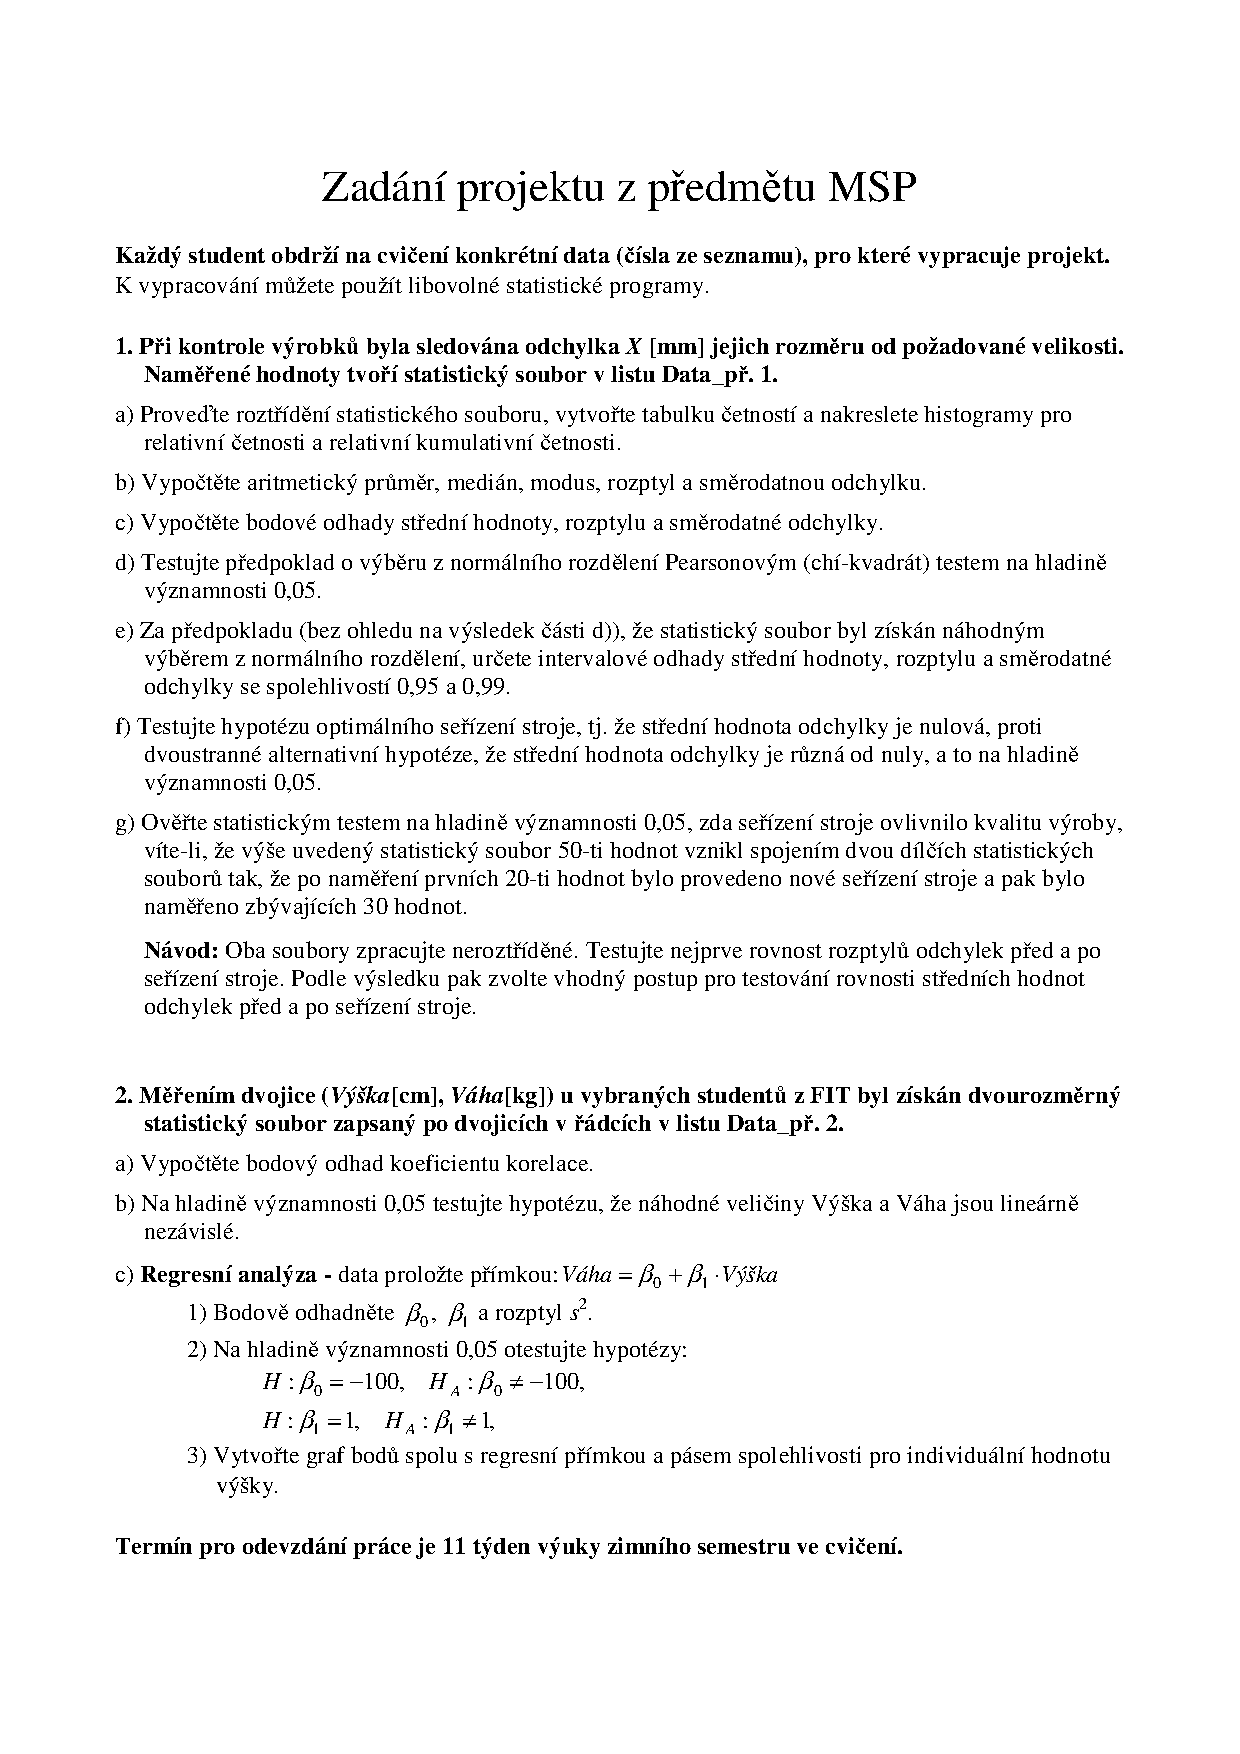
\includepdf{images/zadani.pdf}

%%%%%%%%%%%%%%%%%%%%%%%%%%%%%%%%%%%%%%%%%%%%%%%%%%%%%%%%%%%%%%%%%%%%%

\section*{Příklad 1) Při kontrole výrobků byla sledována odchylka X [mm] jejich rozměru od požadované velikosti. Naměřené hodnoty tvoří statistický soubor v listu Data\_př. 1.}

\begin{figure}[H]
    \centering
    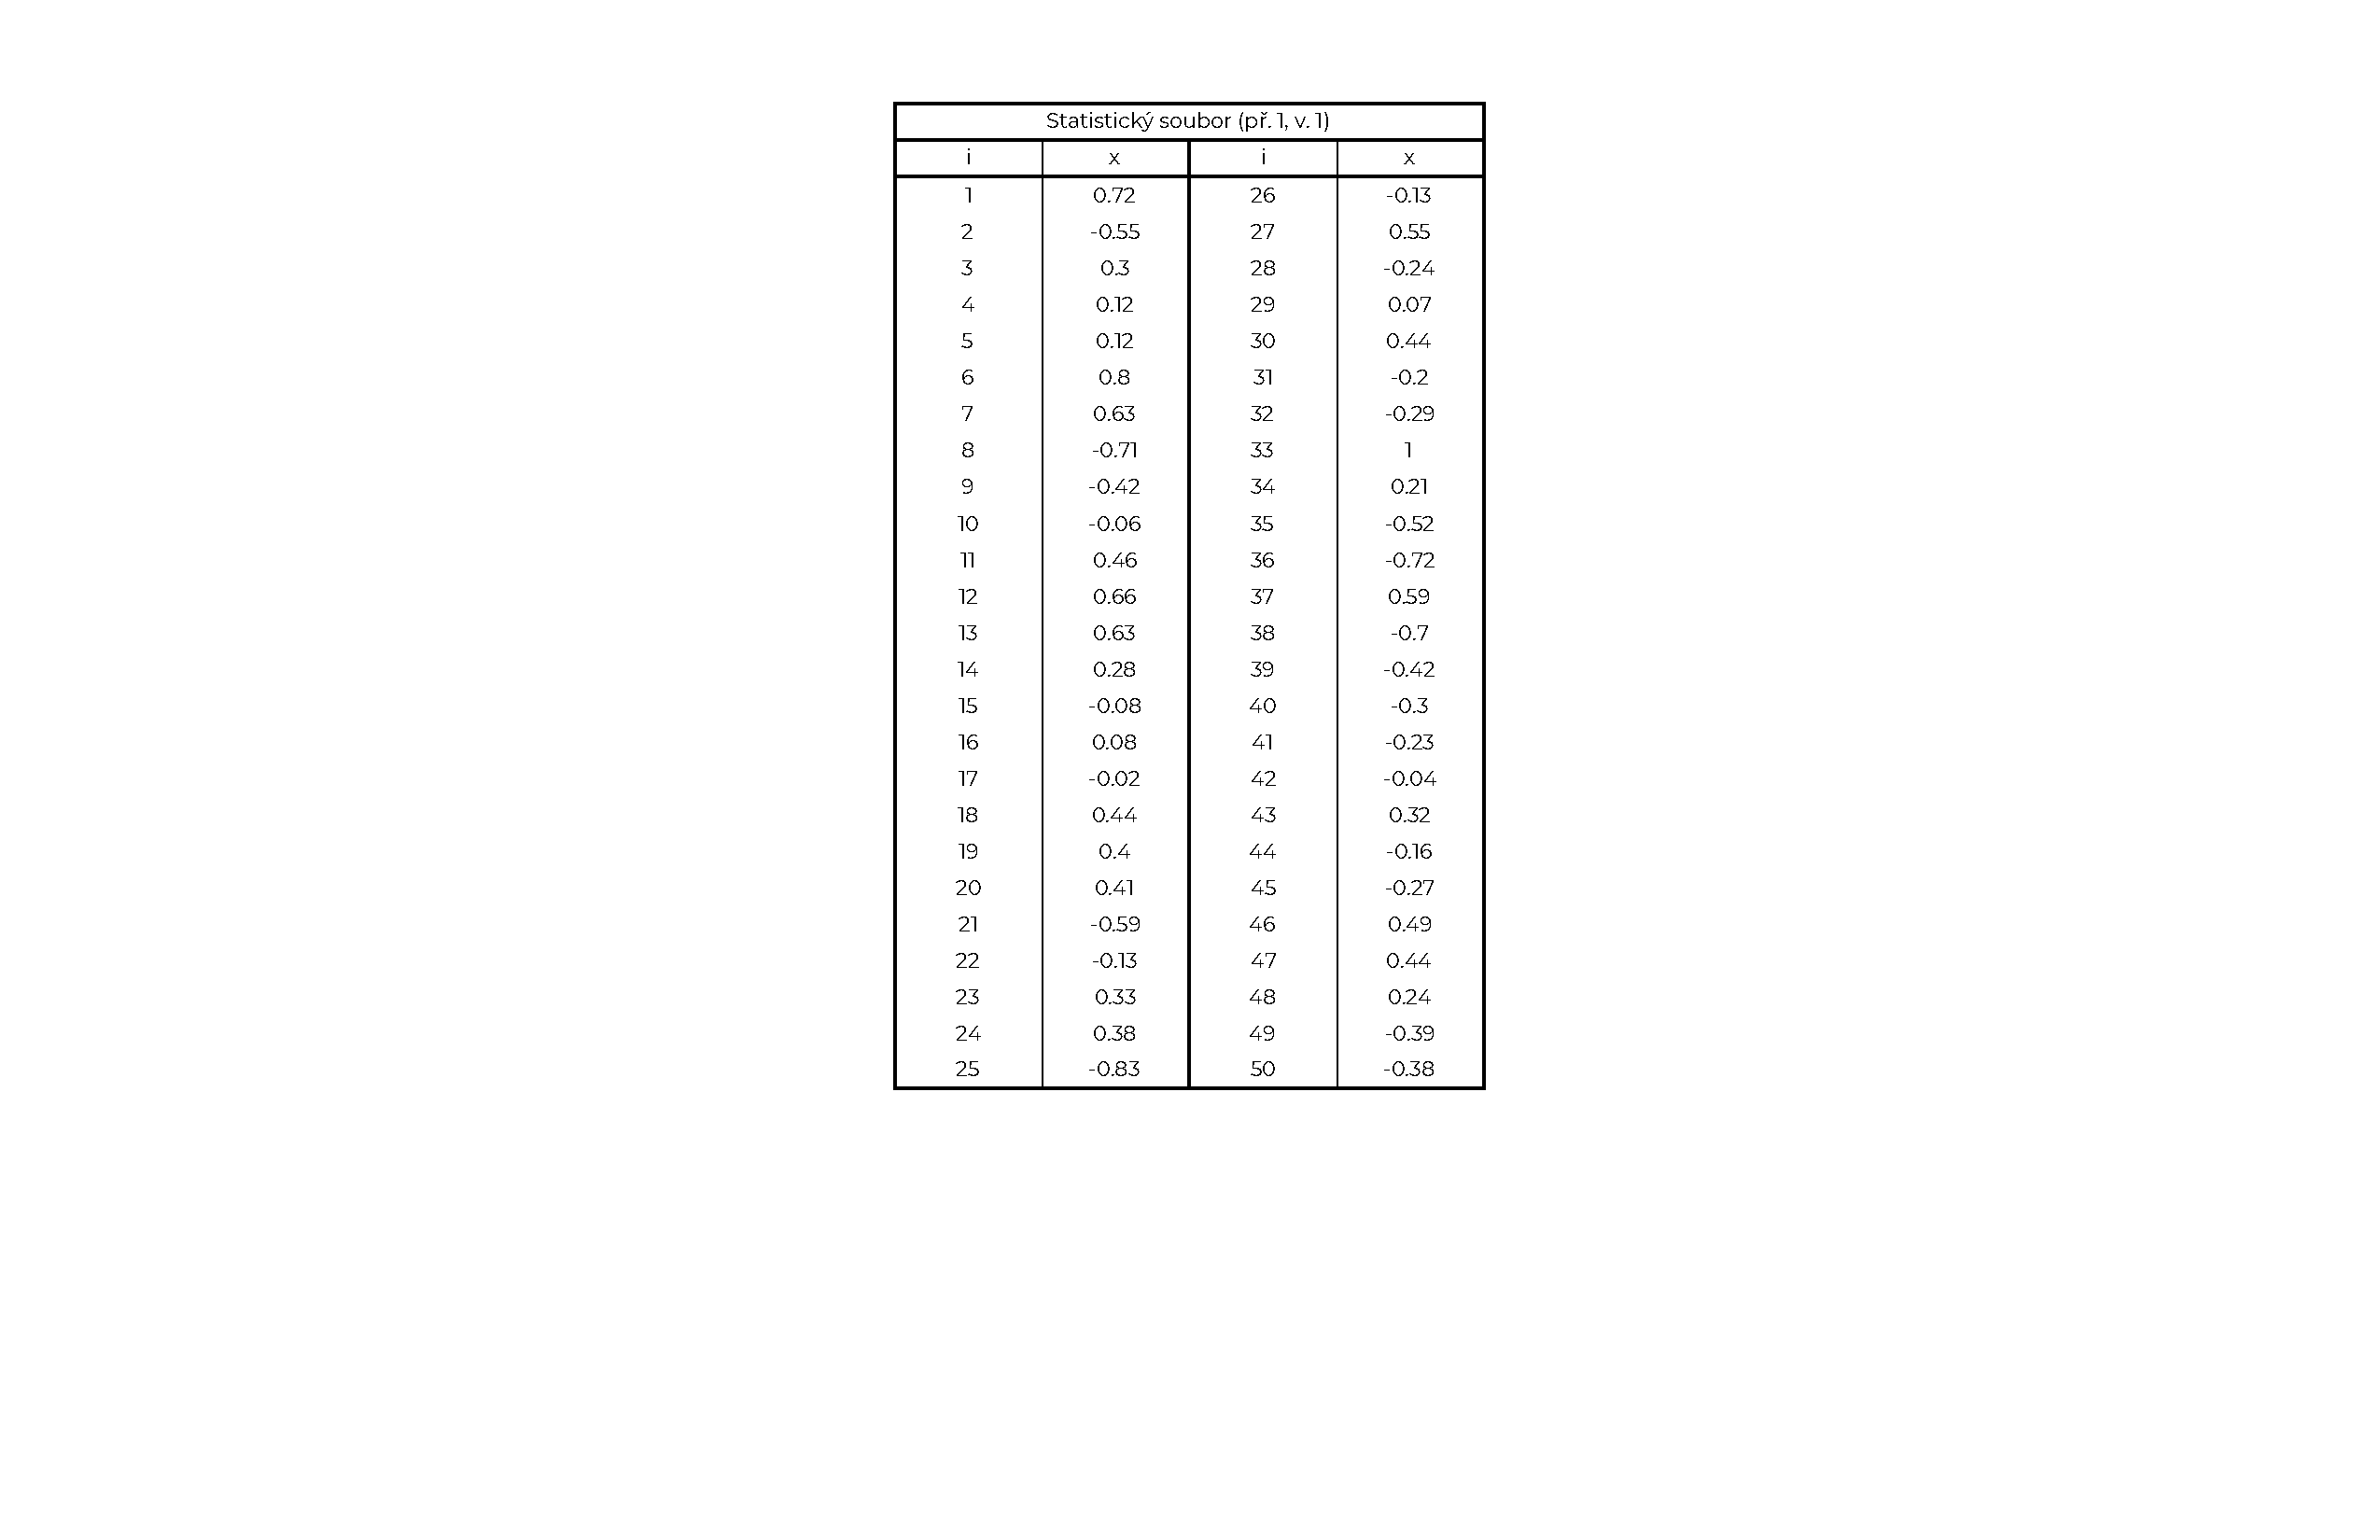
\includegraphics[width=.49\linewidth]{images/1-1-crop.pdf}
    \hfill
    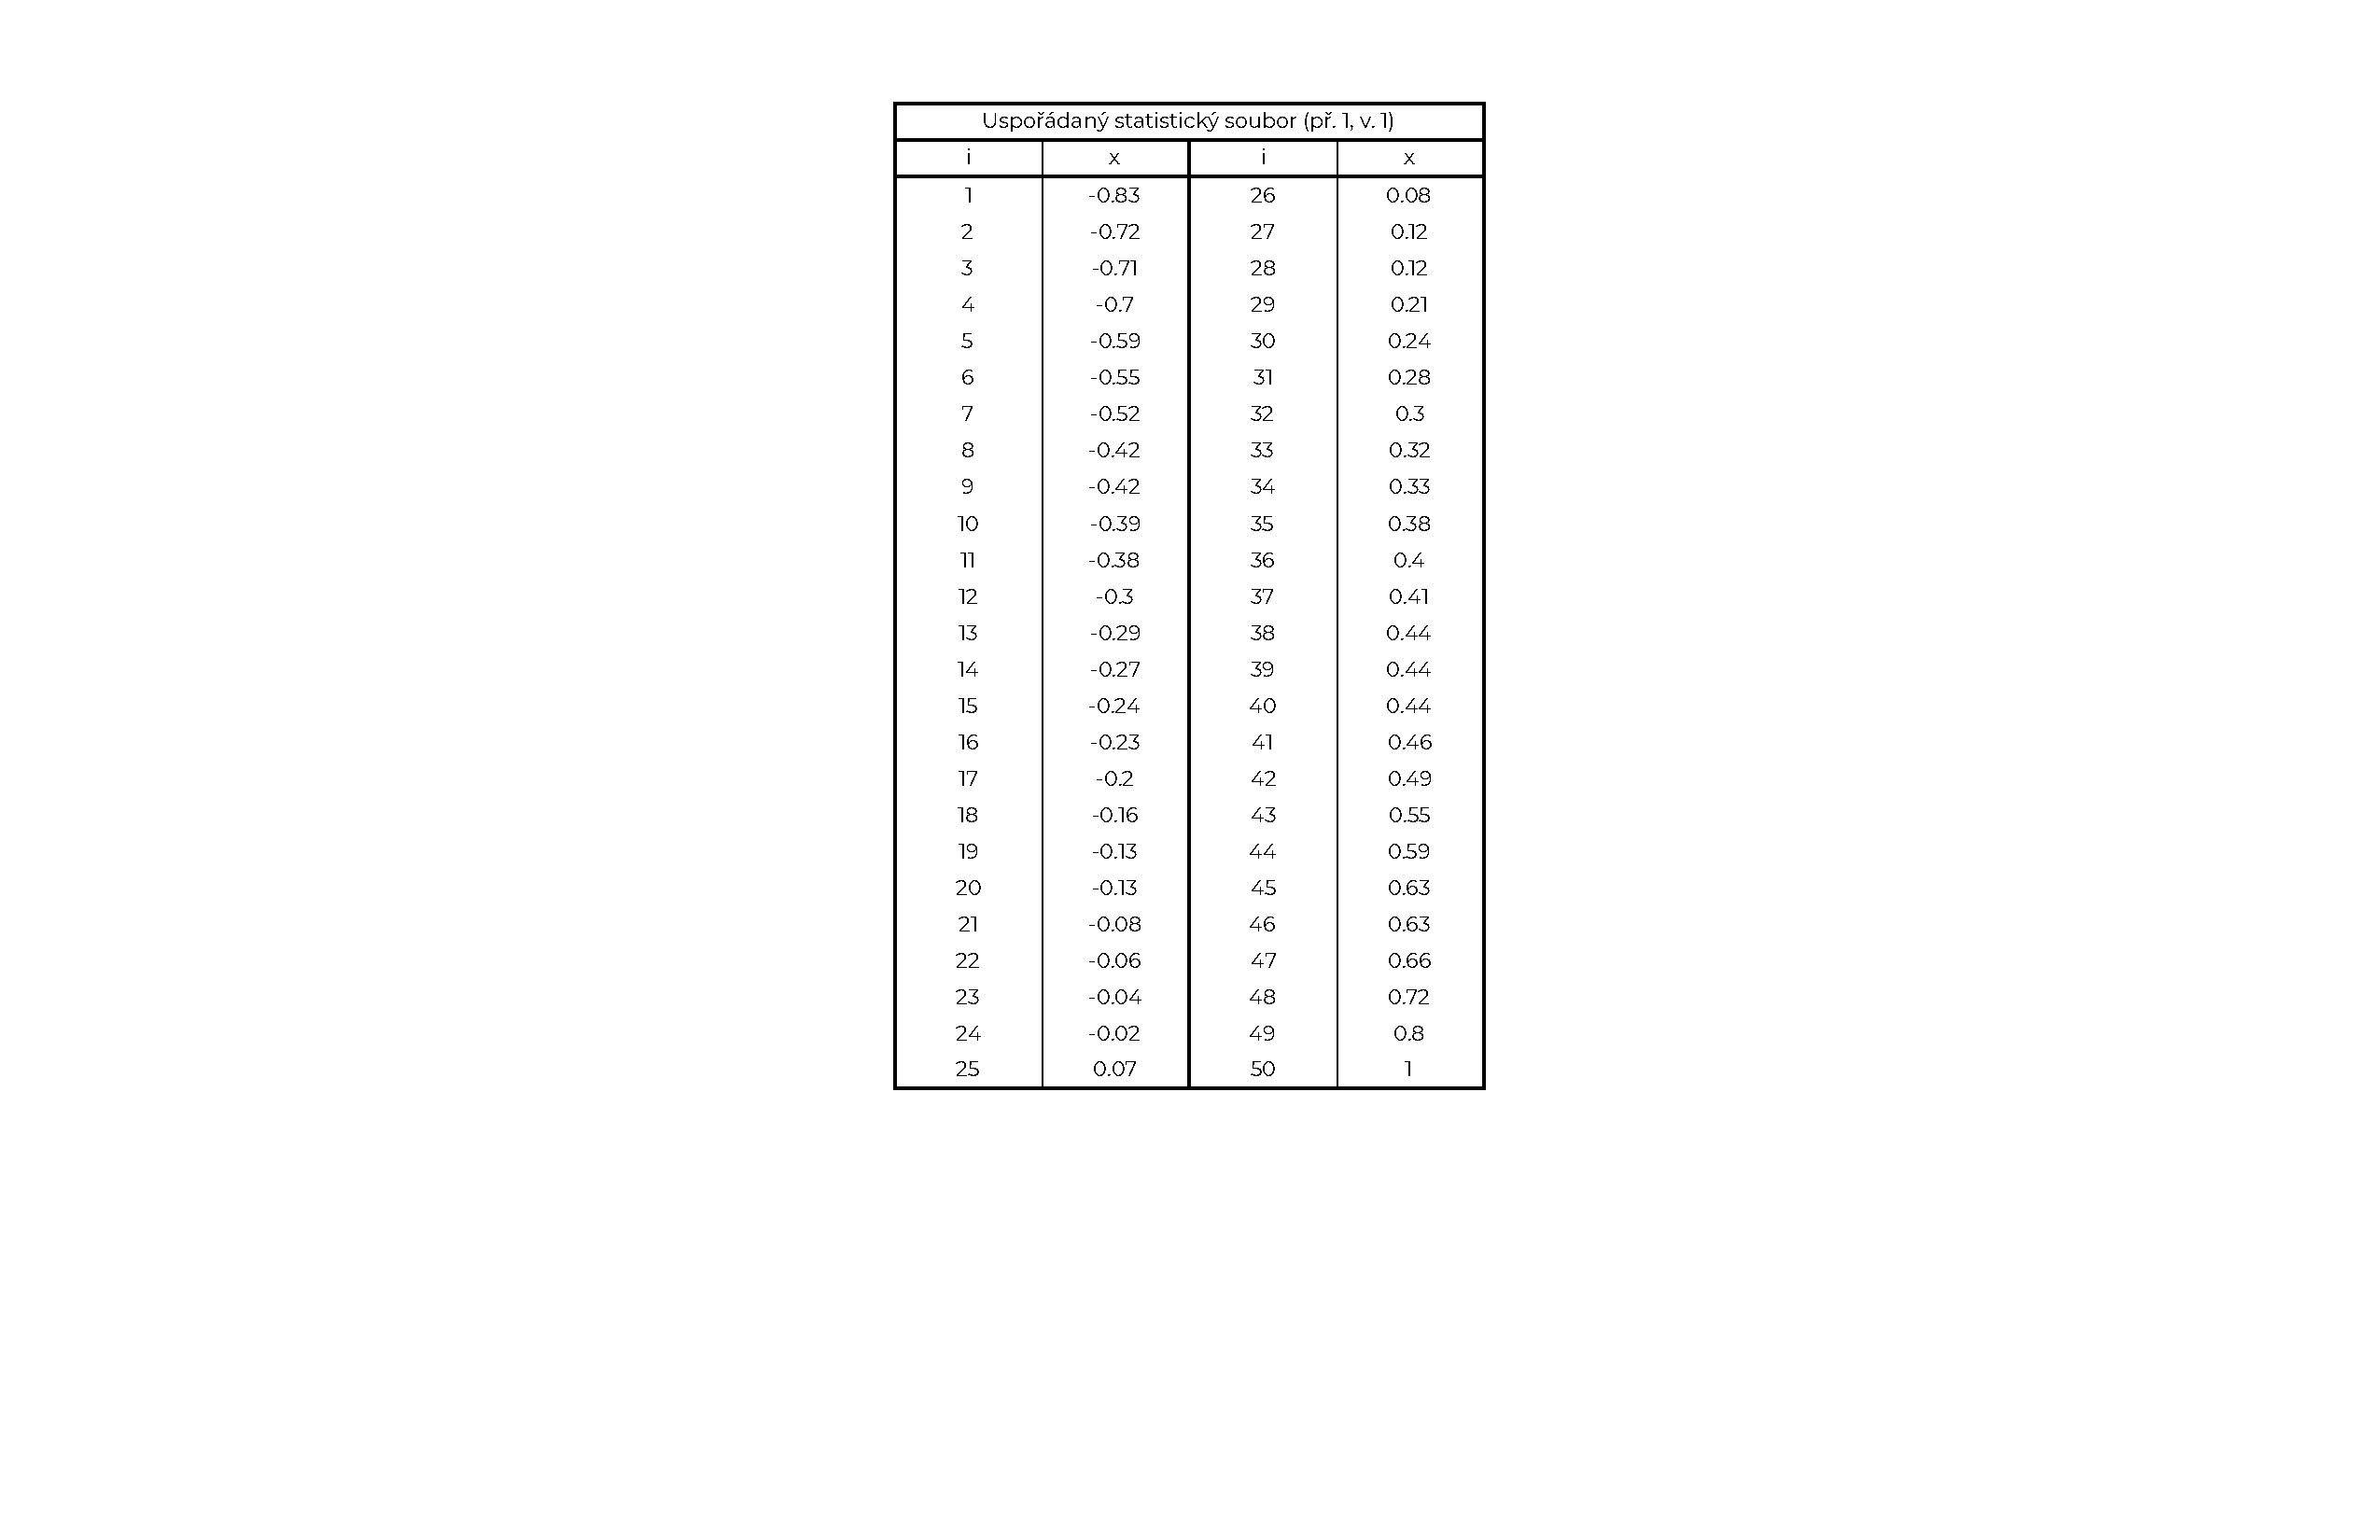
\includegraphics[width=.49\linewidth]{images/1-2-crop.pdf}
\end{figure}

\noindent\makebox[\linewidth]{\rule{\paperwidth}{0.3pt}}

%%%%%%%%%%%%%%%%%%%%%%%%%%%%%%%%%%%%%%%%%%%%%%%%%%%%%%%%%%%%%%%%%%%%%

\subsection*{a) Proveďte roztřídění statistického souboru, vytvořte tabulku četností a nakreslete histogramy pro relativní četnosti a relativní kumulativní četnosti.}
\bigskip

Variační obor: ${\displaystyle \big\langle x_{(1)} \;,\; x_{(n)} \big\rangle = \big\langle \min_{i} x_i \;,\; \max_{i} x_i \big\rangle = \big\langle -0.83 \;,\; 1 \big\rangle}$
\bigskip

Rozpětí: ${\displaystyle x_{(n)} - x_{(1)} = 1.83}$
\bigskip

Počet tříd: ${\displaystyle m = 10}$
\bigskip

Délka třídy: ${\displaystyle \frac{x_{(n)} - x_{(1)}}{m} = 0.183}$


\begin{figure}[H]
    \centering
    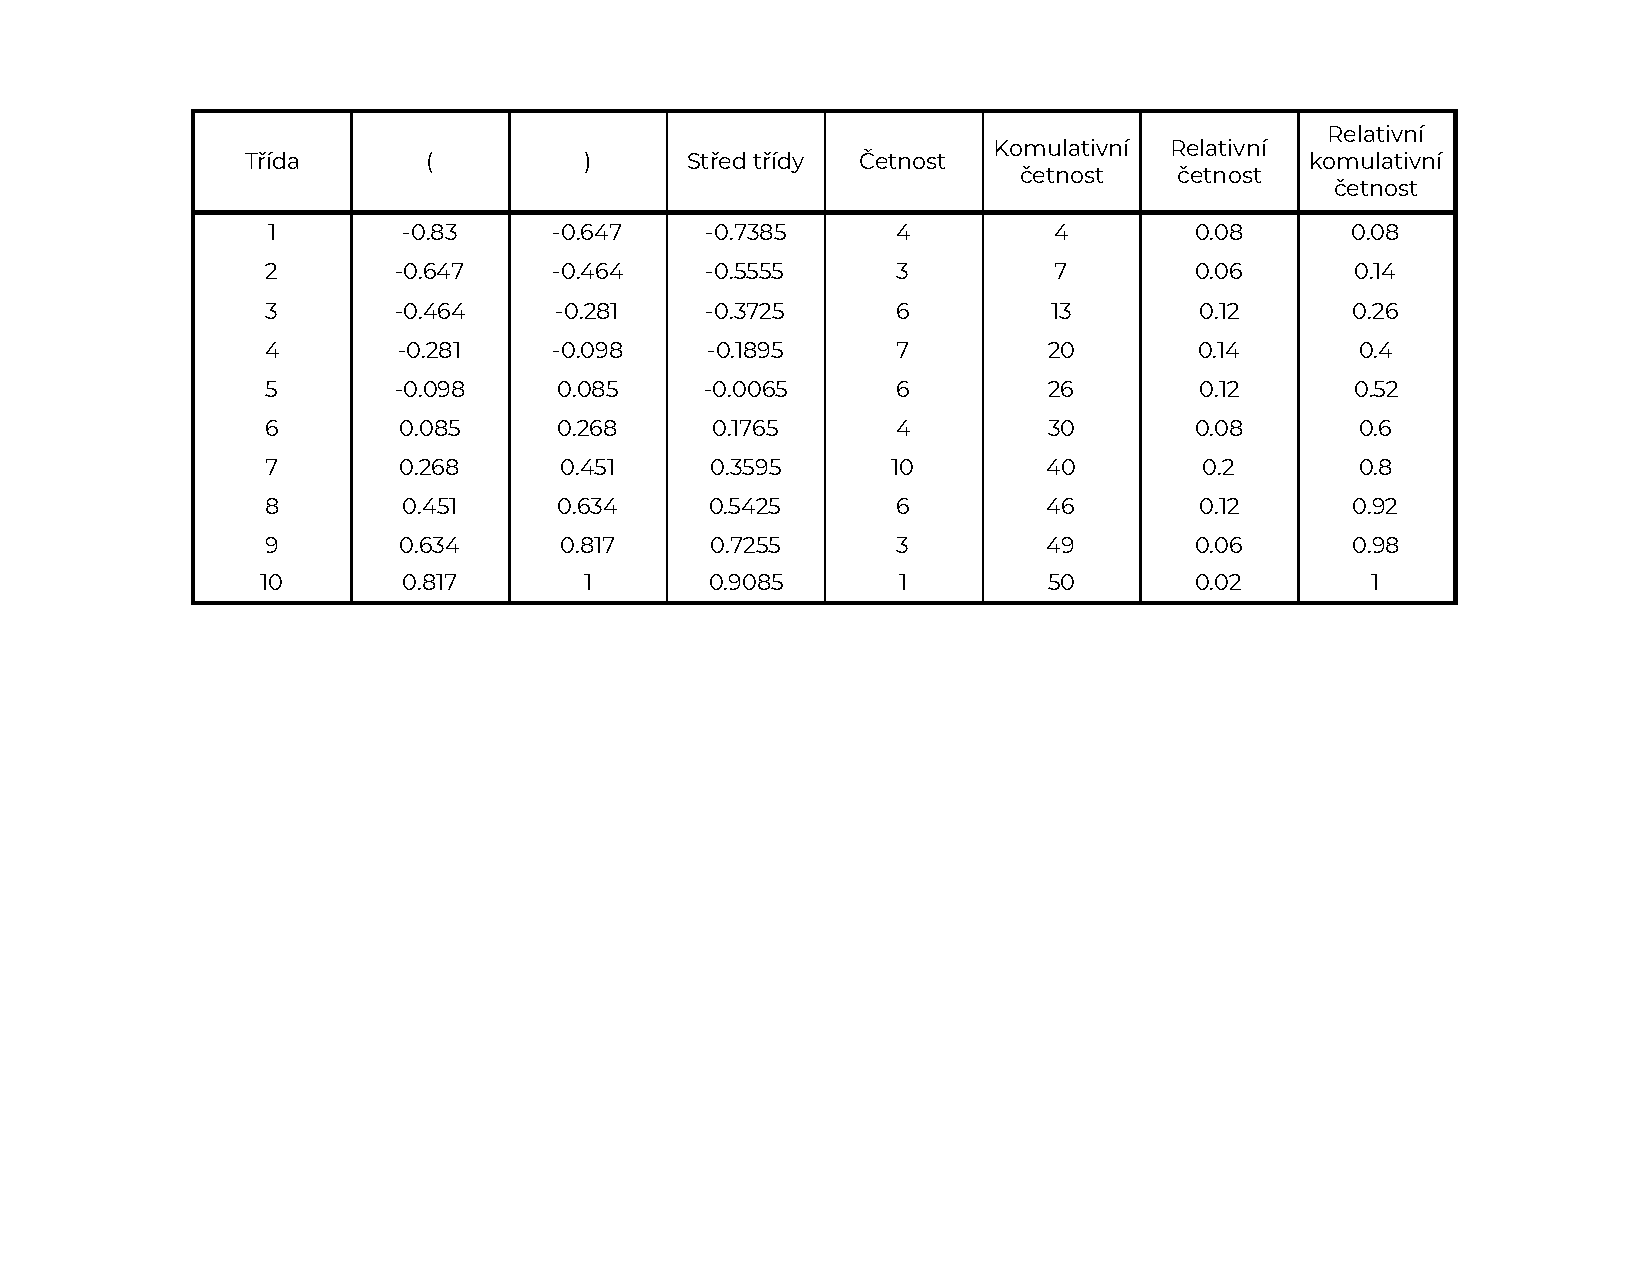
\includegraphics[width=.99\linewidth]{images/1-a-1-crop.pdf}
\end{figure}

\begin{figure}[H]
    \centering
    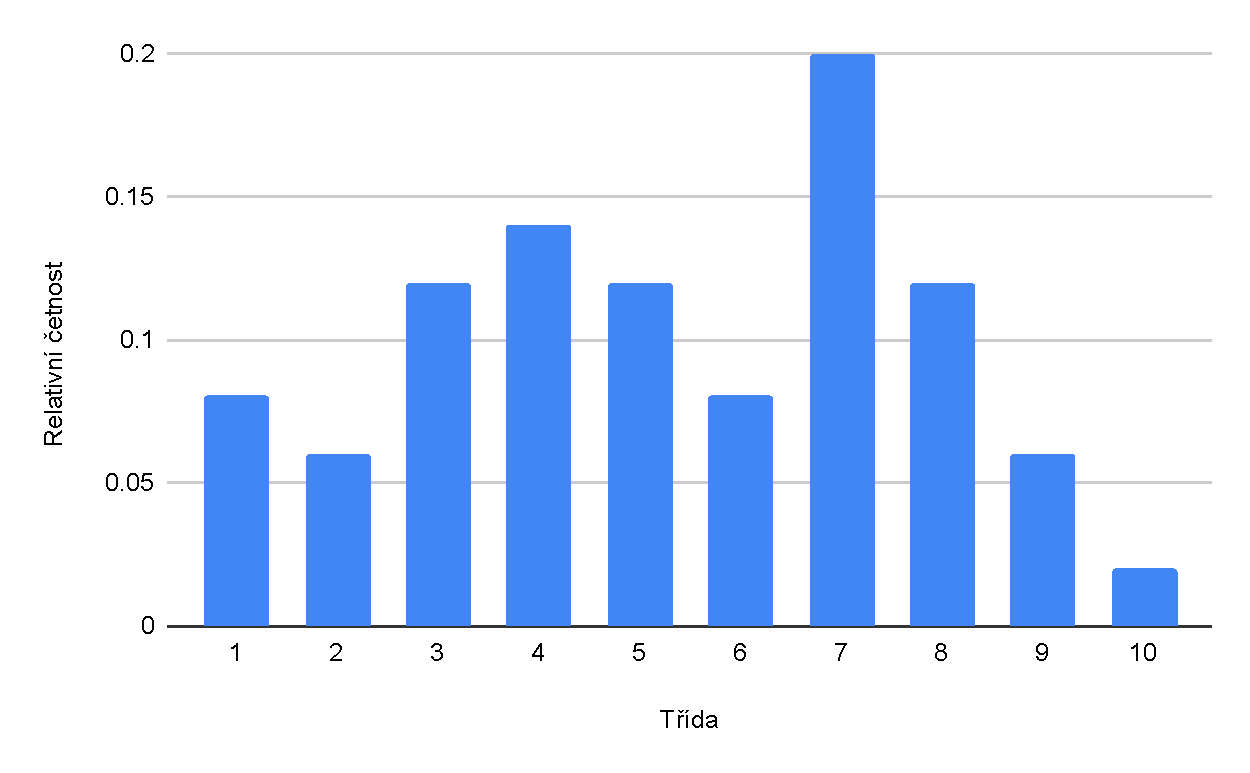
\includegraphics[width=.75\linewidth]{images/1-a-2.pdf}
\end{figure}

\begin{figure}[H]
    \centering
    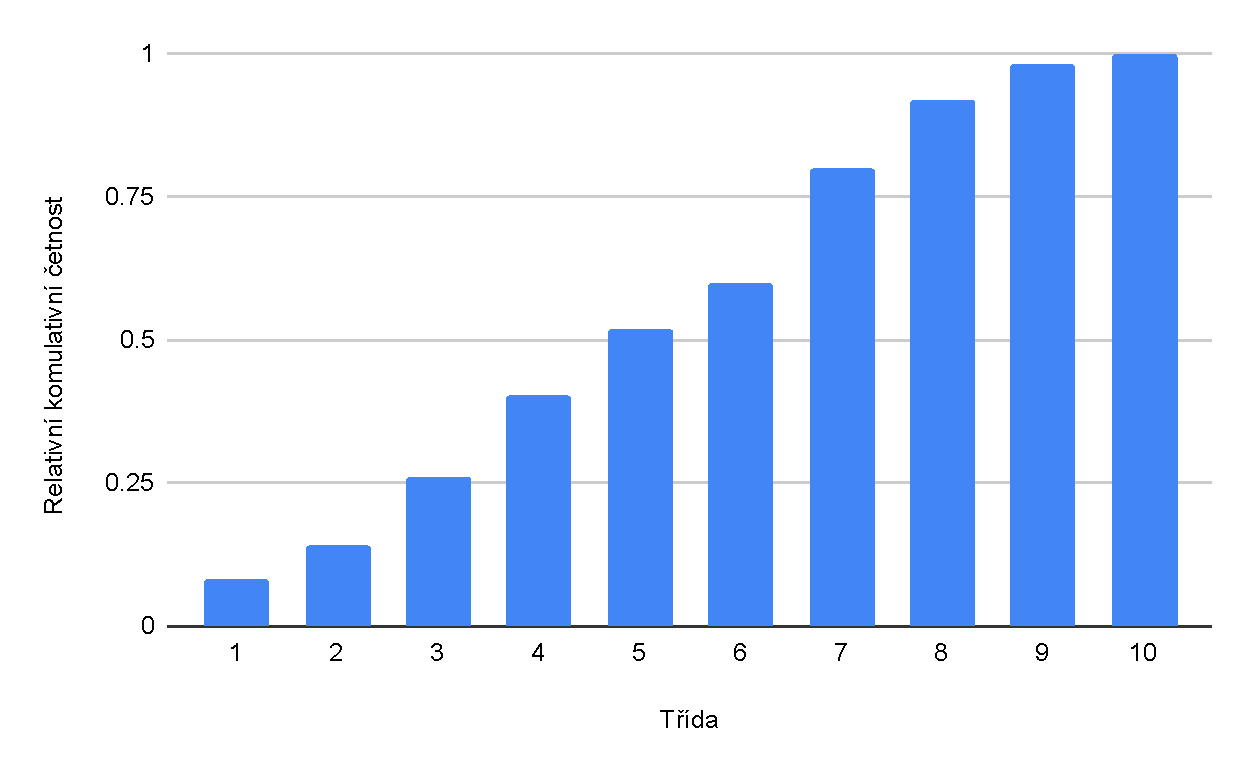
\includegraphics[width=.75\linewidth]{images/1-a-3.pdf}
\end{figure}

\newpage

%%%%%%%%%%%%%%%%%%%%%%%%%%%%%%%%%%%%%%%%%%%%%%%%%%%%%%%%%%%%%%%%%%%%%

\subsection*{b) Vypočtěte aritmetický průměr, medián, modus, rozptyl a směrodatnou odchylku.}

Aritmetický průměr: ${\displaystyle \overline{x} = {\frac {1}{n}} \sum_{i=1}^{n} x_{i} = 0.0546}$
\smallskip

Medián: ${\displaystyle \tilde{x} = 0.075}$
\bigskip

Modus: ${\displaystyle \hat{x} = 0.44}$
\bigskip

Rozptyl: ${\displaystyle s^2 = {\frac {1}{n}} \sum_{i=1}^{n}(x_i - \overline{x})^2} \approx 0.2031$
\smallskip

Směrodatná odchylka: ${\displaystyle s = \sqrt{{\frac {1}{n}} \sum_{i=1}^{n}(x_i - \overline{x})^2}} \approx 0.4507$
\bigskip

\noindent\makebox[\linewidth]{\rule{\paperwidth}{0.3pt}}

%%%%%%%%%%%%%%%%%%%%%%%%%%%%%%%%%%%%%%%%%%%%%%%%%%%%%%%%%%%%%%%%%%%%%

\subsection*{c) Vypočtěte bodové odhady střední hodnoty, rozptylu a směrodatné odchylky.}

Bodový odhad střední hodnoty: ${\displaystyle \overline{x} = {\frac {1}{n}} \sum_{i=1}^{n} x_{i} = 0.0546}$
\bigskip

Bodový odhad rozptylu: ${\displaystyle s^2 = {\frac {1}{n-1}} \sum_{i=1}^{n}(x_i - \overline{x})^2} \approx 0.2073$
\smallskip

Bodový odhad směrodatné odchylky: ${\displaystyle s = \sqrt{{\frac {1}{n-1}} \sum_{i=1}^{n}(x_i - \overline{x})^2}} \approx 0.4553$
\bigskip

\noindent\makebox[\linewidth]{\rule{\paperwidth}{0.3pt}}

%%%%%%%%%%%%%%%%%%%%%%%%%%%%%%%%%%%%%%%%%%%%%%%%%%%%%%%%%%%%%%%%%%%%%

\subsection*{d) Testujte předpoklad o výběru z normálního rozdělení Pearsonovým (chí-kvadrát) testem na hladině významnosti $0.05$.}

\begin{figure}[H]
    \centering
    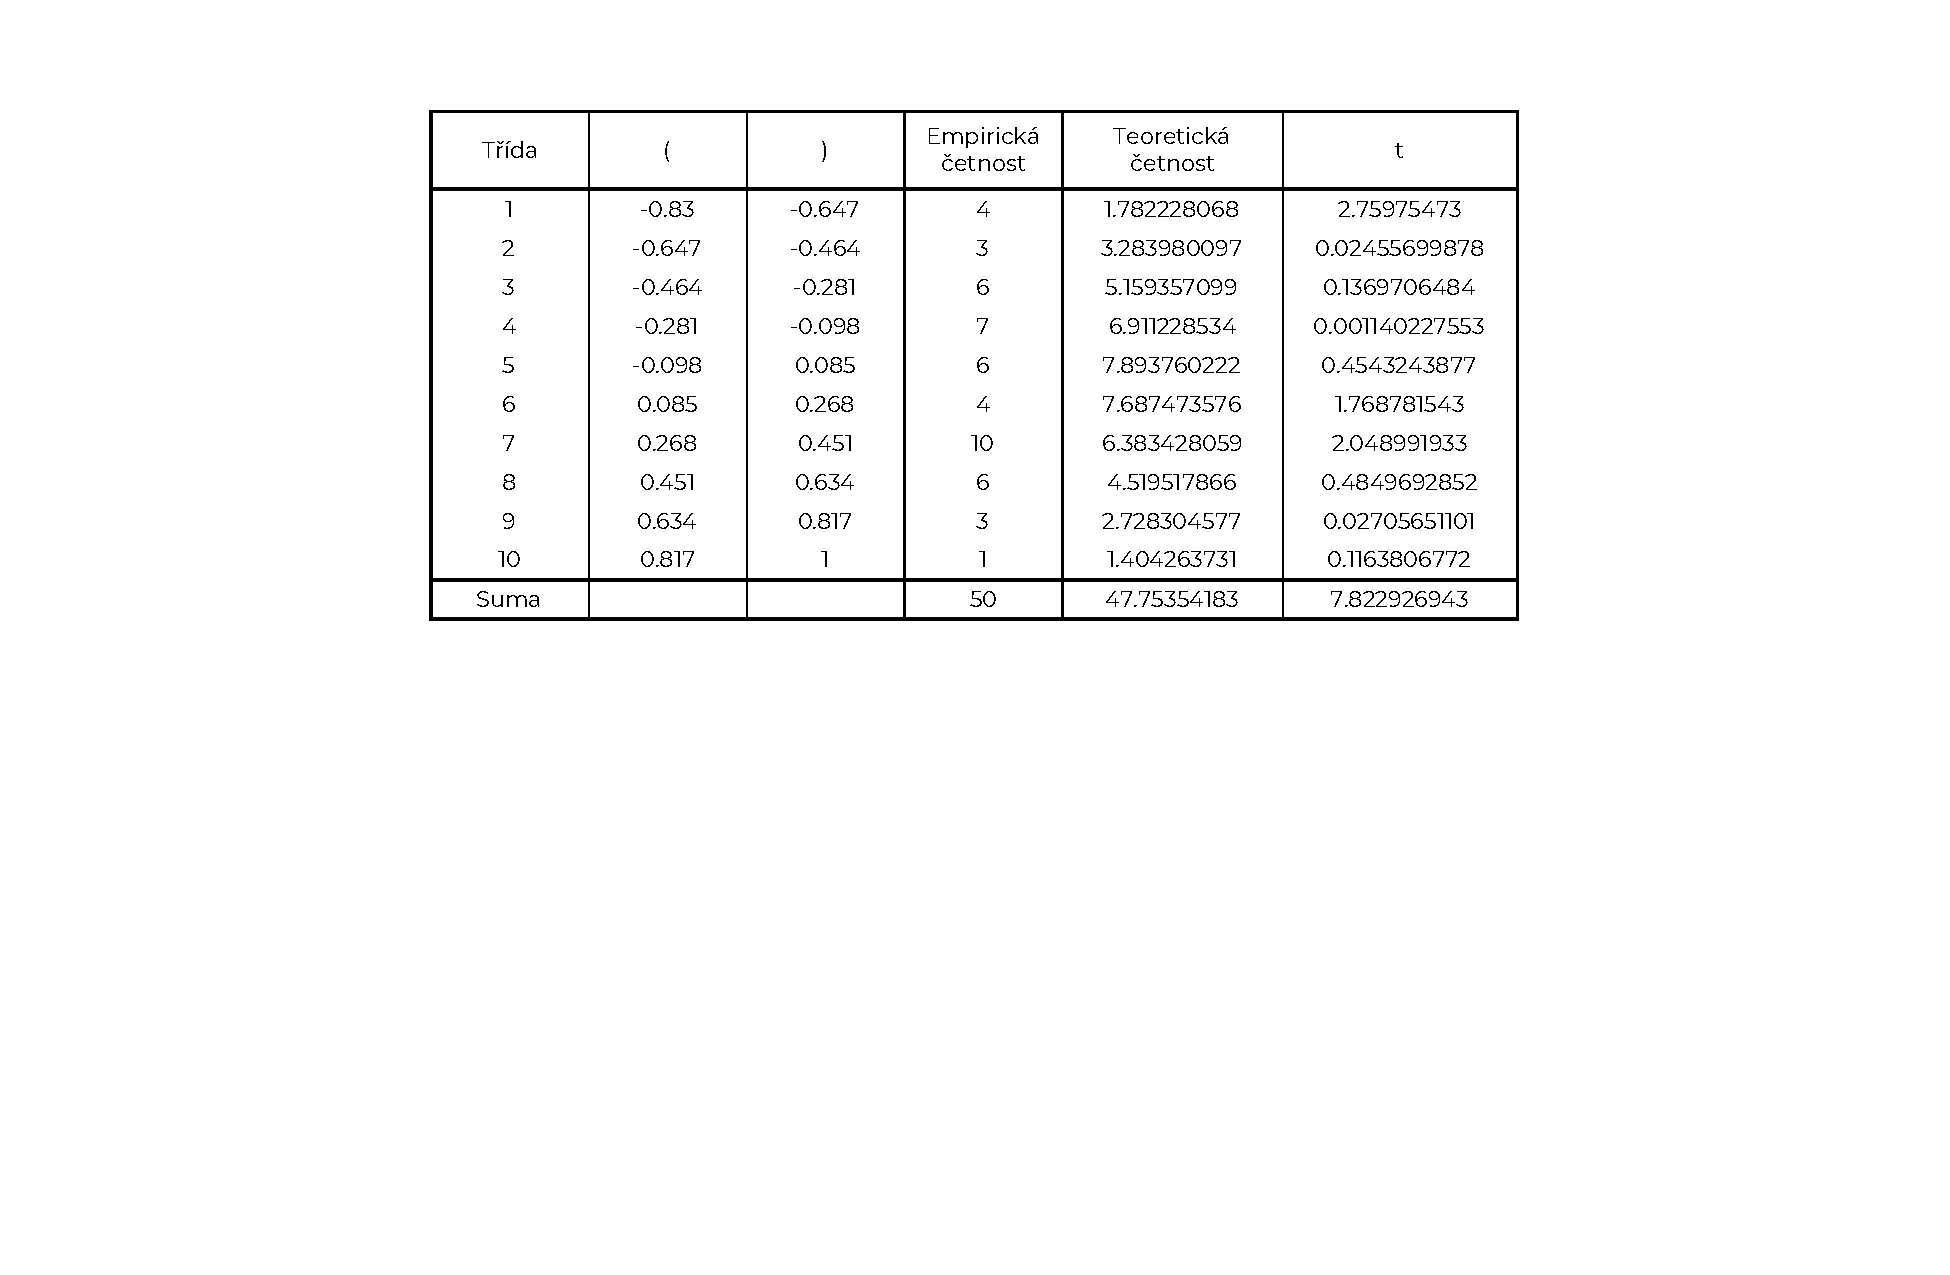
\includegraphics[width=.98\linewidth]{images/1-d-1-crop.pdf}
\end{figure}

Aby celkový počet teoretických četností odpovídal reálným, byly krajní intervaly rozšířeny. Aby všechny teoretické četnosti byly větší jako 1 a aspoň 80\,\% z nich bylo větších než 5 byly hranice tříd upraveny.

\begin{figure}[H]
    \centering
    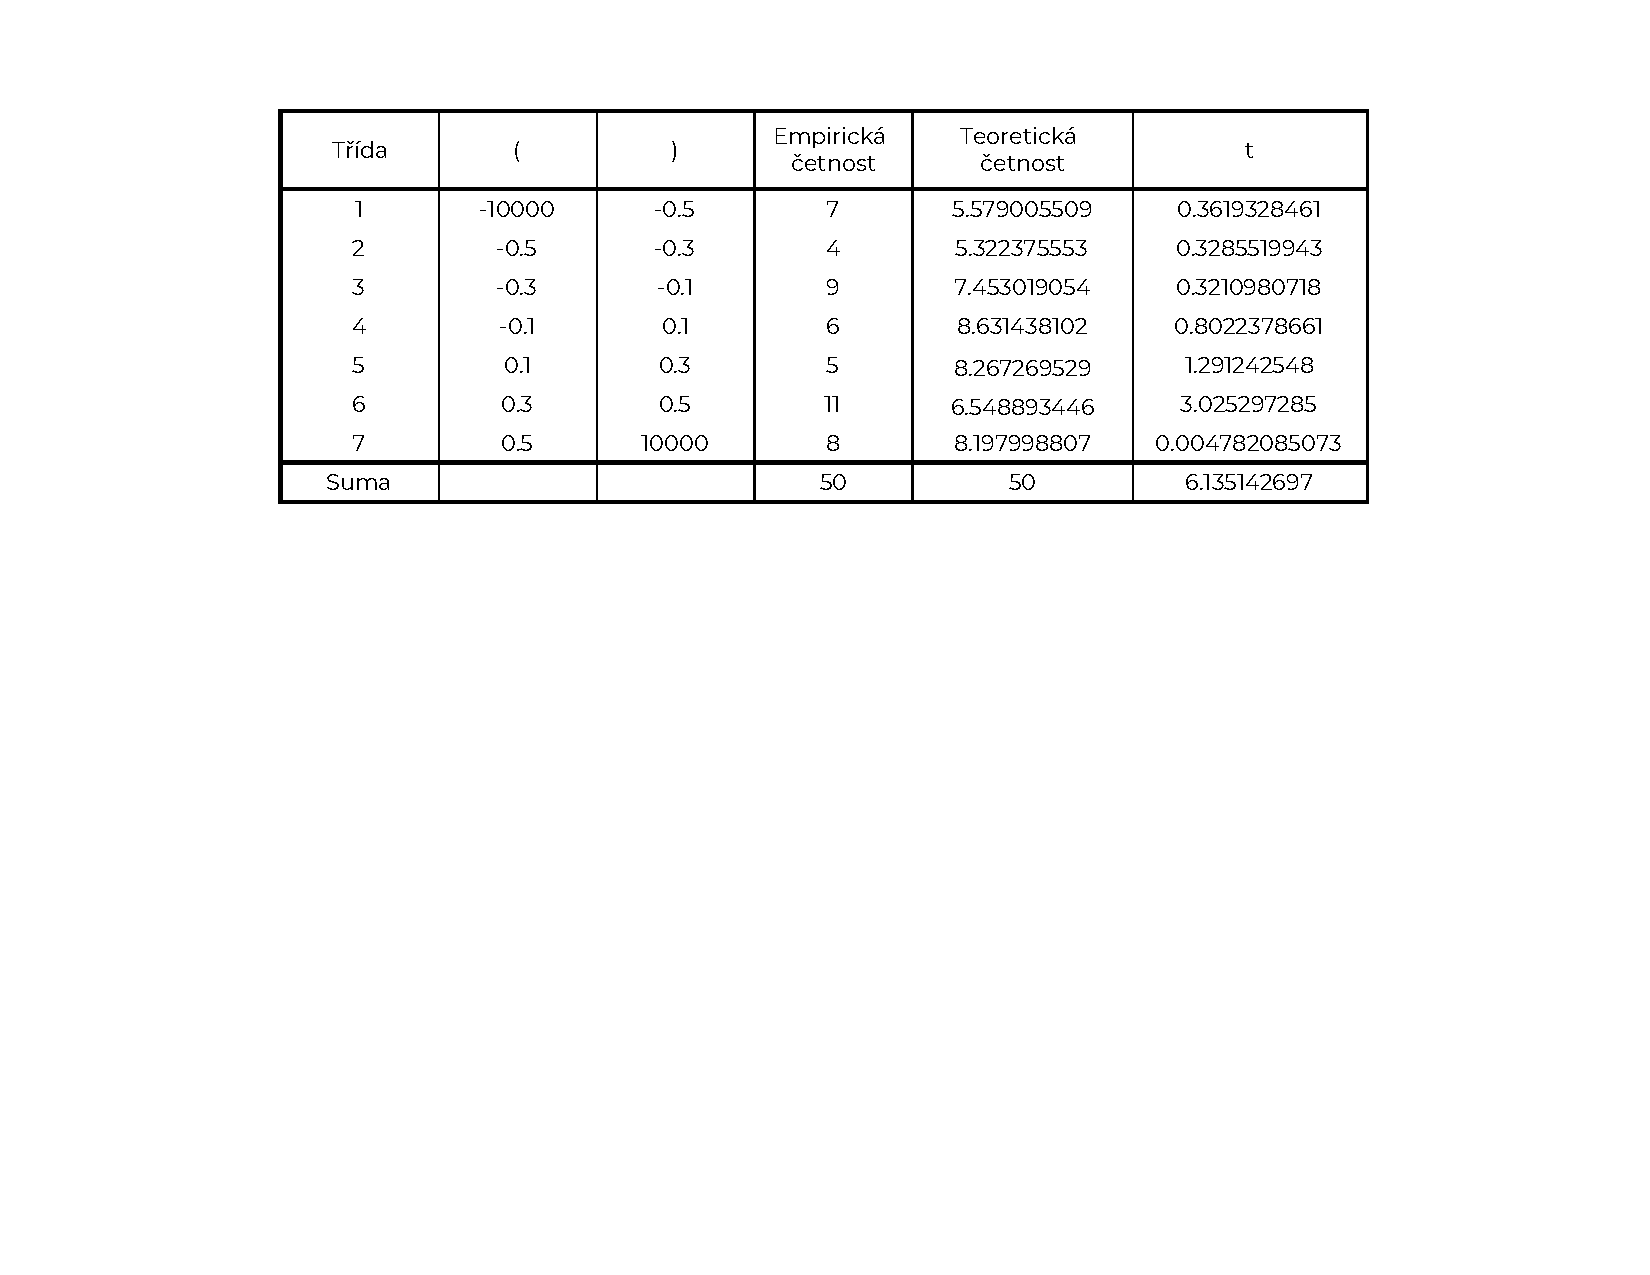
\includegraphics[width=.98\linewidth]{images/1-d-2-crop.pdf}
\end{figure}
\bigskip

Testovací kritérium: ${\displaystyle t = \sum_{i=1}^{m} = \frac{(f_i - \hat{f_i})^2}{\hat{f_i}} \approx 6.135}$, kde $f$ je empirická četnost a $\hat{f}$ je teoretická četnost.
\medskip

Stupeň volnosti: ${\displaystyle k = m - q - 1 = 4}$, kde $m$ je počet tříd a $q$ je počet odhadů parametrů.
\medskip

Kvantil Pearsonova rozdělení pro hladinu významnosti ${\displaystyle \alpha = 0.05}$:
\medskip

${\displaystyle \qquad \chi_{1 - \alpha}^2(k) = \chi_{0.95}^2(4) \approx 9.4877}$
\medskip

Doplněk kritického oboru: ${\displaystyle \overline{W_\alpha} = \big\langle 0 \;,\; \chi_{1 - \alpha}^2(k) \big\rangle \approx \big\langle 0 \;,\; 9.4877 \big\rangle}$
\medskip

Jelikož ${\displaystyle t \in \overline{W_\alpha}}$, tak hypotéza ${\displaystyle X \sim N(0.0546, 0.2073)}$ se \textbf{nezamítá}.
\bigskip

\begin{figure}[H]
    \centering
    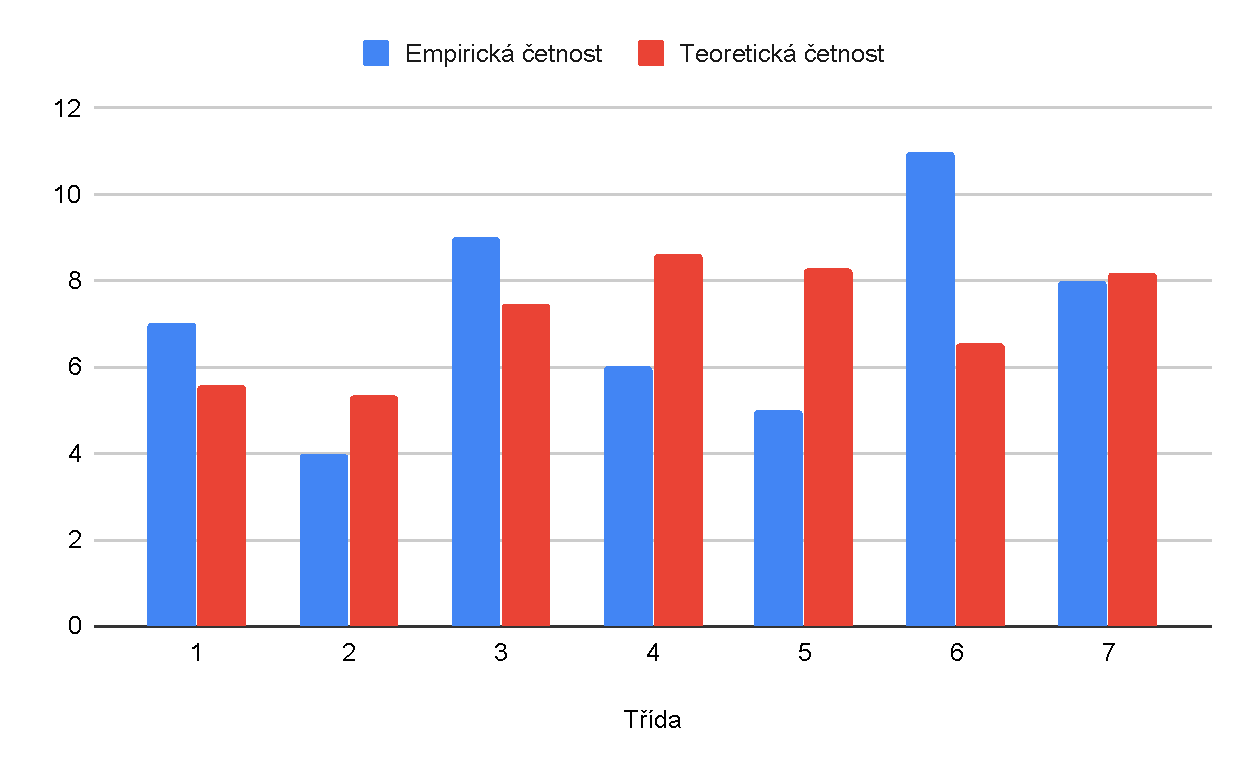
\includegraphics[width=.98\linewidth]{images/1-d-3.pdf}
\end{figure}

\newpage

%%%%%%%%%%%%%%%%%%%%%%%%%%%%%%%%%%%%%%%%%%%%%%%%%%%%%%%%%%%%%%%%%%%%%

\subsection*{e) Za předpokladu (bez ohledu na výsledek části d), že statistický soubor byl získán náhodným výběrem z normálního rozdělení, určete intervalové odhady střední hodnoty, rozptylu a směrodatné odchylky se spolehlivostí $0.95$ a $0.99$.}
\bigskip

Předpokládáme ${\displaystyle X \sim N(\mu, \sigma^2)}$
\medskip

Bodový odhad střední hodnoty: ${\displaystyle \overline{x} = 0.0546}$
\medskip

Bodový odhad rozptylu: ${\displaystyle s^2 \approx 0.2073}$
\medskip

Bodový odhad směrodatné odchylky: ${\displaystyle s \approx 0.4553}$
\bigskip
\bigskip



\textbf{Intervalový odhad střední hodnoty}
\medskip

Stupeň volnosti: ${\displaystyle k = n - 1 = 49}$, kde $n$ je počet vzorků.
\medskip

Kvantil Studentova rozdělení pro hladinu významnosti ${\displaystyle \alpha = 0.05}$:
\medskip

${\displaystyle \qquad t_{1 - \frac{\alpha}{2}}(k) = t_{0.975}(49) \approx 2.0096}$
\medskip

Kvantil Studentova rozdělení pro hladinu významnosti ${\displaystyle \alpha = 0.01}$:
\medskip

${\displaystyle \qquad t_{1 - \frac{\alpha}{2}}(k) = t_{0.995}(49) \approx 2.6799}$
\medskip

Střední hodnota pro ${\displaystyle \alpha = 0.05 :}$
\medskip

% 0.0546 - (2.0096 * (0.4553 / sqrt(49))) = -0.0761
% 0.0546 + (2.0096 * (0.4553 / sqrt(49))) = 0.1853

${\displaystyle \qquad \mu \in \bigg\langle \overline{x} - t_{1 - \frac{\alpha}{2}}(k) \cdot \frac{s}{\sqrt{n}} \;,\; \overline{x} + t_{1 - \frac{\alpha}{2}}(k) \cdot \frac{s}{\sqrt{n}} \bigg\rangle \approx \bigg\langle -0.0761 \;,\; 0.1853 \bigg\rangle}$
\medskip

Střední hodnota pro ${\displaystyle \alpha = 0.01 :}$
\medskip

% 0.0546 - (2.6799 * (0.4553 / sqrt(49))) = -0.1197
% 0.0546 + (2.6799 * (0.4553 / sqrt(49))) = 0.2289

${\displaystyle \qquad \mu \in \bigg\langle \overline{x} - t_{1 - \frac{\alpha}{2}}(k) \cdot \frac{s}{\sqrt{n}} \;,\; \overline{x} + t_{1 - \frac{\alpha}{2}}(k) \cdot \frac{s}{\sqrt{n}} \bigg\rangle \approx \bigg\langle -0.1197 \;,\; 0.2289 \bigg\rangle}$
\bigskip
\bigskip


\textbf{Intervalový odhad rozptylu}
\medskip

Kvantil Pearsonova rozdělení pro hladinu významnosti ${\displaystyle \alpha = 0.05}$:
\medskip

${\displaystyle \qquad \chi_{\frac{\alpha}{2}}^2(k) = \chi_{0.025}^2(49) \approx 31.555}$
\medskip

${\displaystyle \qquad \chi_{1 - \frac{\alpha}{2}}^2(k) = \chi_{0.975}^2(49) \approx  70.222}$
\medskip

Kvantil Pearsonova rozdělení pro hladinu významnosti ${\displaystyle \alpha = 0.01}$:
\medskip

${\displaystyle \qquad \chi_{\frac{\alpha}{2}}^2(k) = \chi_{0.005}^2(49) \approx 27.249}$
\medskip

${\displaystyle \qquad \chi_{1 - \frac{\alpha}{2}}^2(k) = \chi_{0.995}^2(49) \approx  78.231}$
\medskip

Rozptyl pro ${\displaystyle \alpha = 0.05 :}$
\medskip

% (49*0.2073)/70.222 = 0.1447
% (49*0.2073)/31.555 = 0.3219

${\displaystyle \qquad \sigma^2 \in \bigg\langle \frac{(n - 1) \cdot s^2}{\chi_{1 - \frac{\alpha}{2}}^2(k)} \;,\; \frac{(n - 1) \cdot s^2}{\chi_{\frac{\alpha}{2}}^2(k)} \bigg\rangle \approx \bigg\langle 0.1447 \;,\; 0.3219 \bigg\rangle}$
\medskip

Rozptyl pro ${\displaystyle \alpha = 0.01 :}$
\medskip

% (49*0.2073)/78.231 = 0.1298
% (49*0.2073)/27.249 = 0.3727

${\displaystyle \qquad \sigma^2 \in \bigg\langle \frac{(n - 1) \cdot s^2}{\chi_{1 - \frac{\alpha}{2}}^2(k)} \;,\; \frac{(n - 1) \cdot s^2}{\chi_{\frac{\alpha}{2}}^2(k)} \bigg\rangle \approx \bigg\langle 0.1298 \;,\; 0.3727 \bigg\rangle}$
\newpage



\textbf{Intervalový odhad směrodatné odchylky}
\medskip

Směrodatná odchylka pro ${\displaystyle \alpha = 0.05 :}$
\medskip

% sqrt((49*0.2073)/70.222) = 0.3803
% sqrt((49*0.2073)/31.555) = 0.5674

${\displaystyle \qquad \sigma \in \bigg\langle \sqrt{\frac{(n - 1) \cdot s^2}{\chi_{1 - \frac{\alpha}{2}}^2(k)}} \;,\; \sqrt{\frac{(n - 1) \cdot s^2}{\chi_{\frac{\alpha}{2}}^2(k)}} \bigg\rangle \approx \bigg\langle 0.3803 \;,\; 0.5674 \bigg\rangle}$
\bigskip

Směrodatná odchylka pro ${\displaystyle \alpha = 0.01 :}$
\medskip

% sqrt((49*0.2073)/78.231) = 0.3603
% sqrt((49*0.2073)/27.249) = 0.6106

${\displaystyle \qquad \sigma \in \bigg\langle \sqrt{\frac{(n - 1) \cdot s^2}{\chi_{1 - \frac{\alpha}{2}}^2(k)}} \;,\; \sqrt{\frac{(n - 1) \cdot s^2}{\chi_{\frac{\alpha}{2}}^2(k)}} \bigg\rangle \approx \bigg\langle 0.3603 \;,\; 0.6106 \bigg\rangle}$
\bigskip
\medskip

\noindent\makebox[\linewidth]{\rule{\paperwidth}{0.3pt}}

%%%%%%%%%%%%%%%%%%%%%%%%%%%%%%%%%%%%%%%%%%%%%%%%%%%%%%%%%%%%%%%%%%%%%

\subsection*{f) Testujte hypotézu optimálního seřízení stroje, tj. že střední hodnota odchylky je nulová, proti dvoustranné alternativní hypotéze, že střední hodnota odchylky je různá od nuly, a to na hladině významnosti $0.05$.}
\medskip



Hypotéza: ${\displaystyle H_0 : \mu = 0}$
\medskip

Alternativní hypotéza ${\displaystyle H_{A} : \mu \neq 0}$
\medskip

Bodový odhad střední hodnoty: ${\displaystyle \overline{x} = 0.0546}$
\medskip

Bodový odhad směrodatné odchylky: ${\displaystyle s \approx 0.4553}$
\medskip

Počet vzorků: ${\displaystyle n = 50}$
\bigskip
\smallskip



\textbf{Testujeme pomocí Studentova jednovýběrového testu}
\medskip

Testovací kritérium: ${\displaystyle t = \frac{\overline{x} - \mu}{s} \cdot \sqrt{n} \approx 0.848}$
\medskip

Stupeň volnosti: ${\displaystyle k = n - 1 = 49}$
\medskip

Kvantil Studentova rozdělení pro hladinu významnosti ${\displaystyle \alpha = 0.05}$:
\medskip

${\displaystyle \qquad t_{1 - \frac{\alpha}{2}}(k) = t_{0.975}(49) \approx 2.0096}$
\medskip

Doplněk kritického oboru pro alternativní hypotézu ${\displaystyle H_{A}}$:
\medskip

${\displaystyle \qquad \overline{W_\alpha} = \big\langle -t_{1 - \frac{\alpha}{2}}(k) \;,\; t_{1 - \frac{\alpha}{2}}(k) \big\rangle \approx \big\langle 2.0096 \;,\; 2.0096 \big\rangle}$
\bigskip
\smallskip



Jelikož ${\displaystyle t \in \overline{W_\alpha}}$, tak hypotéza ${\displaystyle H_0}$ se \textbf{nezamítá} a alternativní hypotéza ${\displaystyle H_A}$ se \textbf{zamítá}.
\bigskip

\newpage

%%%%%%%%%%%%%%%%%%%%%%%%%%%%%%%%%%%%%%%%%%%%%%%%%%%%%%%%%%%%%%%%%%%%%

\subsection*{g) Ověřte statistickým testem na hladině významnosti $0.05$, zda seřízení stroje ovlivnilo kvalitu výroby, víte-li, že výše uvedený statistický soubor $50$ hodnot vznikl spojením dvou dílčích statistických souborů tak, že po naměření prvních $20$ hodnot bylo provedeno nové seřízení stroje a pak bylo naměřeno zbývajících $30$ hodnot.}
\bigskip

\begin{figure}[H]
    \centering
    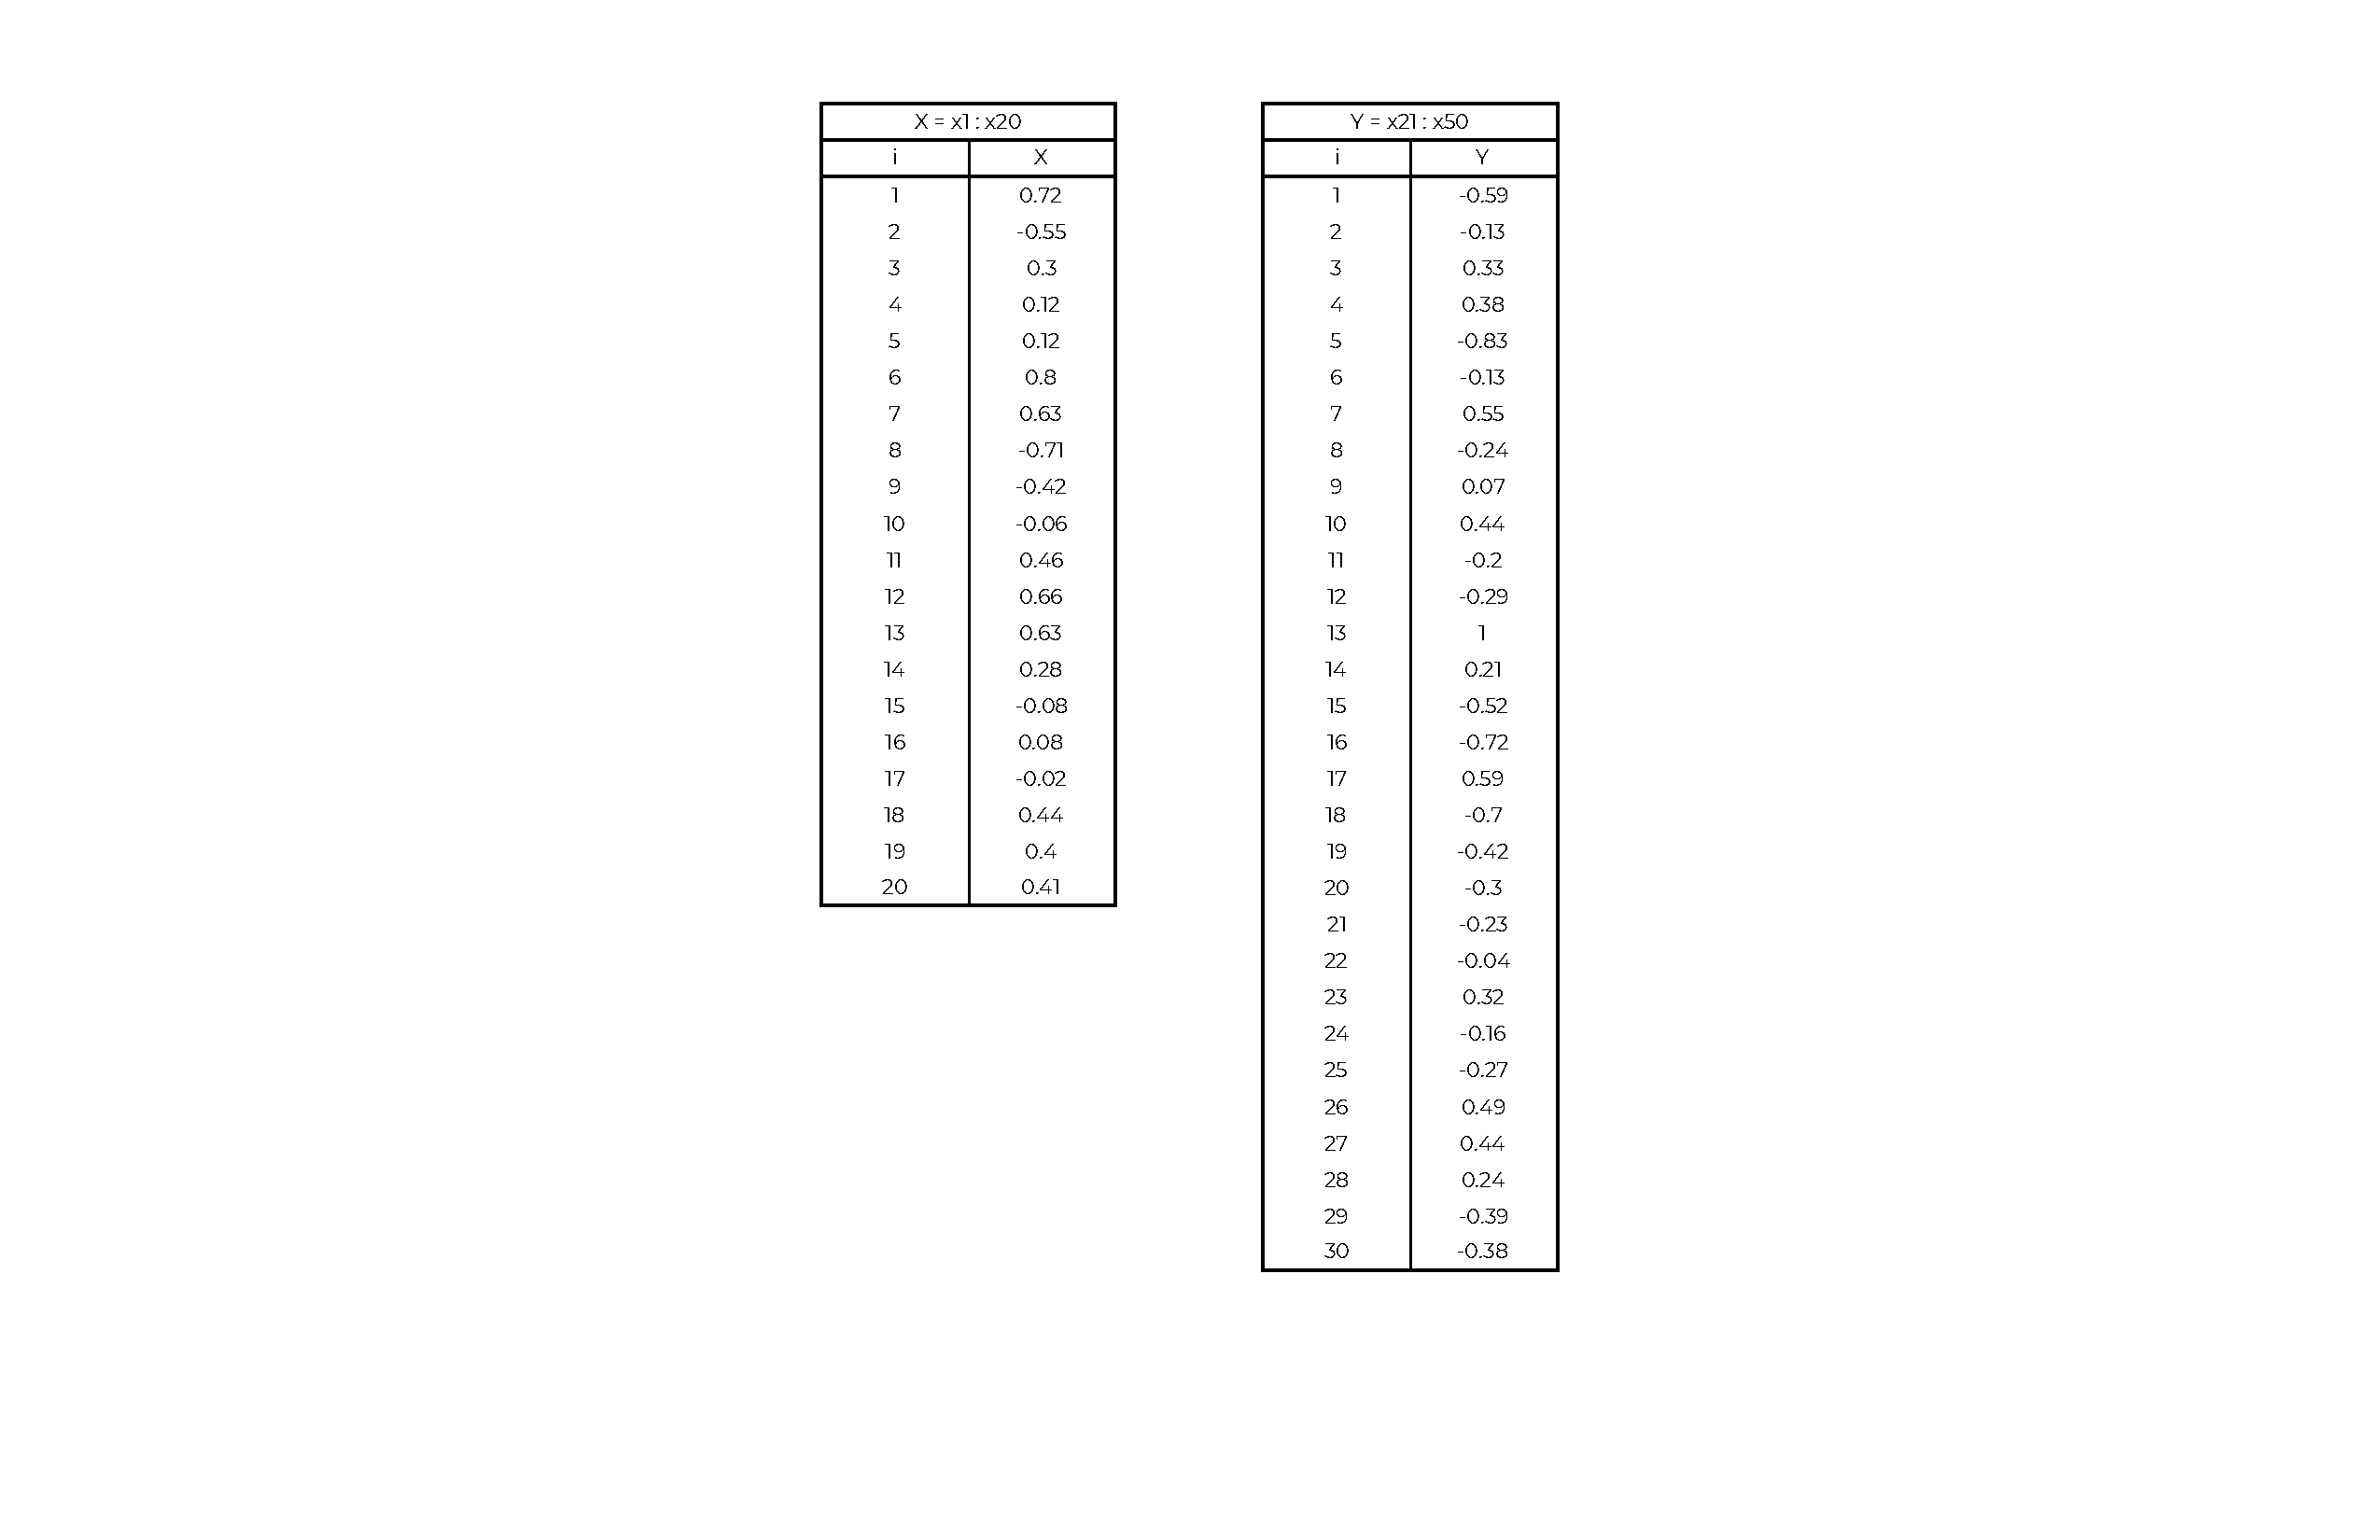
\includegraphics[width=.7\linewidth]{images/1-g-1-crop.pdf}
\end{figure}

\newpage

\begin{minipage}{0.49\textwidth}
    ${\displaystyle n_x = 20}$
    \medskip

    ${\displaystyle \overline{x} = 0.2105}$
    \medskip

    ${\displaystyle s_x^2 \approx 0.1806}$
    \medskip

    ${\displaystyle s_x \approx 0.425}$
\end{minipage}
%
\begin{minipage}{0.49\textwidth}
    ${\displaystyle n_y = 30}$
    \medskip

    ${\displaystyle \overline{y} \approx -0.0493}$
    \medskip

    ${\displaystyle s_y^2 \approx 0.2039}$
    \medskip

    ${\displaystyle s_y \approx 0.4516}$
\end{minipage}
\bigskip
\bigskip



\textbf{Test rovnosti rozptylů pomocí F-testu}
\medskip

Hypotéza ${\displaystyle H_0 : \sigma_x^2 = \sigma_y^2}$
\medskip

Alternativní hypotéza ${\displaystyle H_A : \sigma_x^2 \neq \sigma_y^2}$
\medskip

Testovací kritérium: ${\displaystyle t = \frac{s_x^2}{s_y^2} \approx 0.7844}$
\medskip

Stupně volnosti:
\medskip

${\displaystyle \qquad k_x = n_x - 1 = 19}$
\medskip

${\displaystyle \qquad k_y = n_y - 1 = 29}$
\medskip

Kvantily Fisher-Snedecorova rozdělení pro hladinu významnosti ${\displaystyle \alpha = 0.05}$:
\medskip

${\displaystyle \qquad F_{\frac{\alpha}{2}} (k_x, k_y) = F_{0.025} (19, 29) \approx 0.4163}$
\medskip

${\displaystyle \qquad F_{1 - \frac{\alpha}{2}} (k_x, k_y) = F_{0.975} (19, 29) \approx 2.2313}$
\medskip

Doplněk kritického oboru pro alternativní hypotézu ${\displaystyle H_A}$:
\medskip

${\displaystyle \qquad \overline{W_\alpha} = \big\langle F_{\frac{\alpha}{2}} (k_x, k_y) \;,\; F_{1 - \frac{\alpha}{2}} (k_x, k_y) \big\rangle \approx \big\langle 0.4163 \;,\; 2.2313 \big\rangle}$
\medskip

Jelikož ${\displaystyle t \in \overline{W_\alpha}}$, tak hypotéza ${\displaystyle H_0}$ se \textbf{nezamítá}.
\bigskip
\bigskip



\textbf{Test rovnosti středních hodnot pomocí Studentova dvouvýběrového testu}
\medskip

Hypotéza ${\displaystyle H_0 : \mu_x - \mu_y = \mu_0}$ pro ${\displaystyle \mu_0 = 0}$ za podmínky ${\displaystyle \sigma_x^2 = \sigma_y^2}$
\medskip

Alternativní hypotéza ${\displaystyle H_A : \mu_x - \mu_y \neq 0}$
\medskip

Stupeň volnosti: ${\displaystyle k = n_x + n_y -2 = 48}$
\medskip

Testovací kritérium: ${\displaystyle t = \frac{\overline{x} - \overline{y} - \mu_0}{\sqrt{k_x \cdot s_x^2 + k_y \cdot s_y^2}} \cdot \sqrt{\frac{n_x \cdot n_y \cdot k}{n_x + n_y}} \approx 2.04}$
\medskip

Kvantil Studentova rozdělení pro hladinu významnosti ${\displaystyle \alpha = 0.05}$:
\medskip

${\displaystyle \qquad t_{1 - \frac{\alpha}{2}}(k) = t_{0.975}(48) \approx 2.0106}$
\medskip

Doplněk kritického oboru pro alternativní hypotézu ${\displaystyle H_{A}}$:
\medskip

${\displaystyle \qquad \overline{W_\alpha} = \big\langle -t_{1 - \frac{\alpha}{2}}(k) \;,\; t_{1 - \frac{\alpha}{2}}(k) \big\rangle \approx \big\langle -2.0106 \;,\; 2.0106 \big\rangle}$
\medskip

Jelikož ${\displaystyle t \notin \overline{W_\alpha}}$, tak hypotéza ${\displaystyle H_0}$ se \textbf{zamítá}.

\newpage

%%%%%%%%%%%%%%%%%%%%%%%%%%%%%%%%%%%%%%%%%%%%%%%%%%%%%%%%%%%%%%%%%%%%%

\section*{Příklad 2) Měřením dvojice (Výška[cm], Váha[kg]) u vybraných studentů z FIT byl získán dvourozměrný statistický soubor zapsaný po dvojicích v řádcích v listu Data\_př. 2.}

\begin{figure}[H]
    \centering
    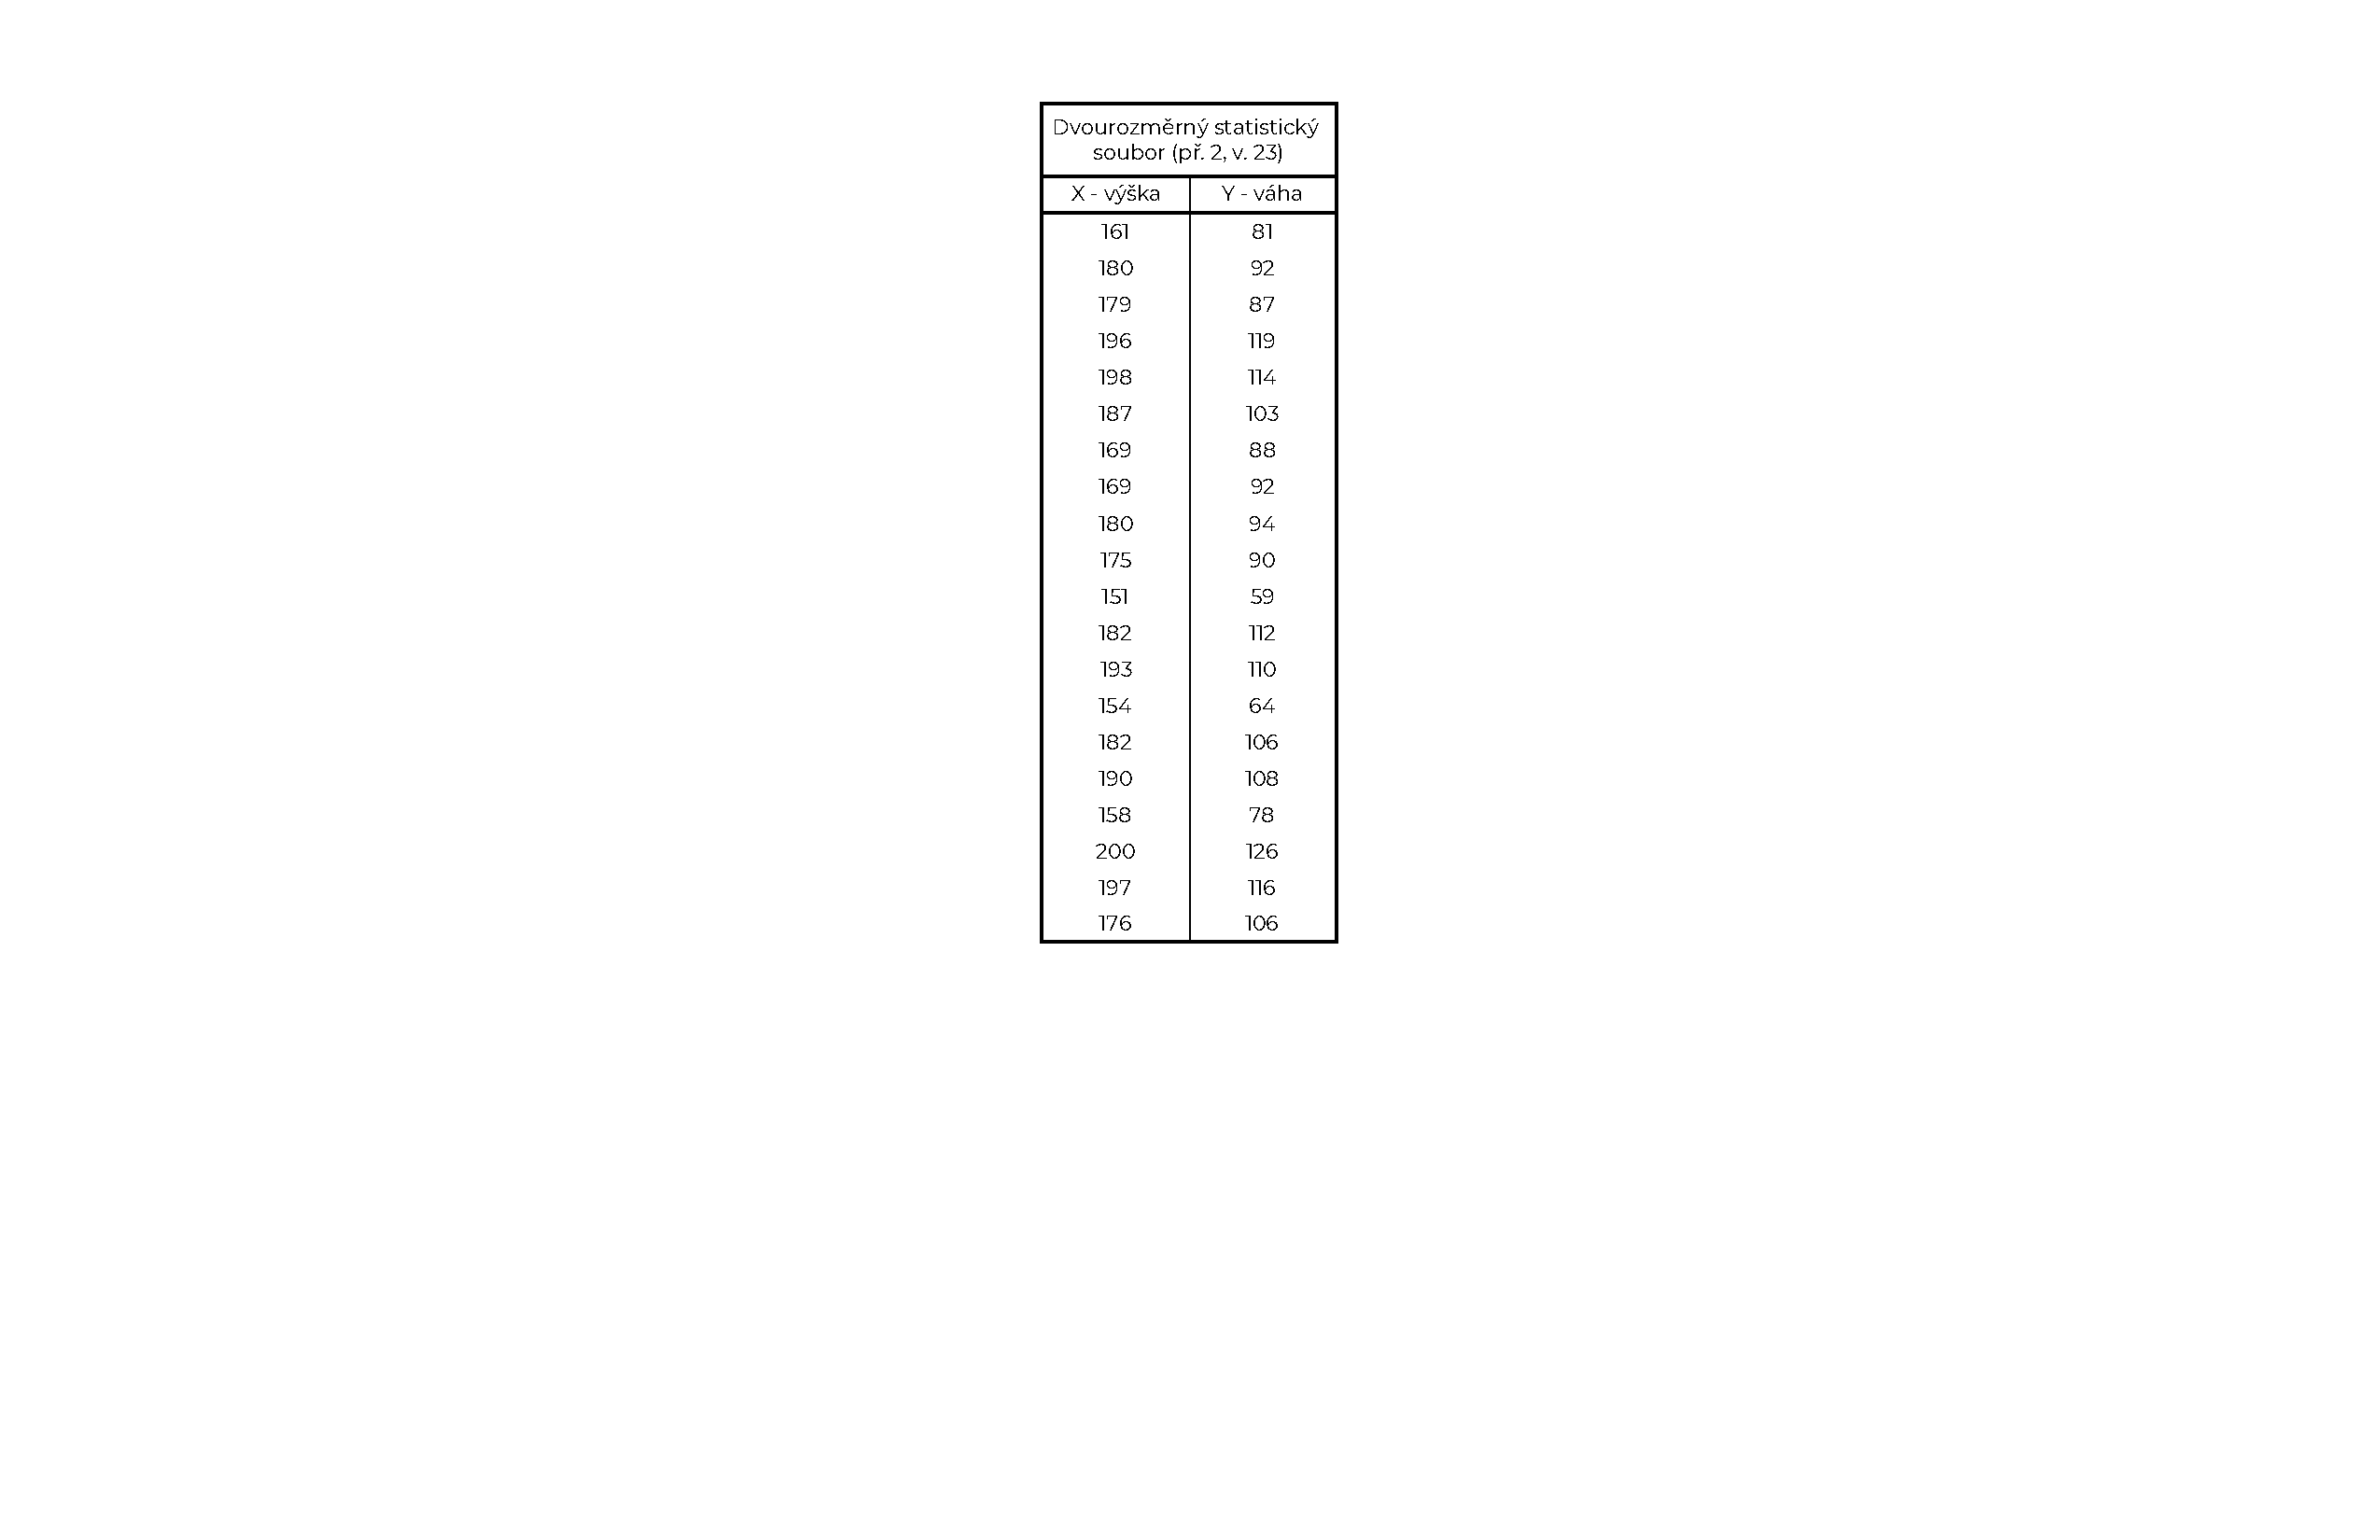
\includegraphics[width=.25\linewidth]{images/2-1-crop.pdf}
\end{figure}

\noindent\makebox[\linewidth]{\rule{\paperwidth}{0.3pt}}

%%%%%%%%%%%%%%%%%%%%%%%%%%%%%%%%%%%%%%%%%%%%%%%%%%%%%%%%%%%%%%%%%%%%%

\subsection*{a) Vypočtěte bodový odhad koeficientu korelace.}
\bigskip

\begin{minipage}{0.49\textwidth}
    ${\displaystyle n = 20}$
    \medskip

    ${\displaystyle \overline{x} = 178.85}$
    \medskip

    ${\displaystyle \overline{y} = 97.25}$
\end{minipage}
%
\begin{minipage}{0.49\textwidth}
    ${\displaystyle \sum_{i=1}^n x_i^2 = 643 \, 961}$
    \medskip

    ${\displaystyle \sum_{i=1}^n y_i^2 = 195 \, 277}$
    \medskip

    ${\displaystyle \sum_{i=1}^n x_i \cdot y_i = 352 \, 644}$
\end{minipage}
\bigskip

Odhad koeficientu korelace: ${\displaystyle r = \frac{\sum\limits_{i=1}^n x_i \cdot y_i - n \cdot \overline{x} \cdot \overline{y}} {\sqrt{ \bigg( \sum\limits_{i=1}^n x_i^2 - n \cdot \overline{x}^2\bigg) \cdot \bigg( \sum\limits_{i=1}^n y_i^2 - n \cdot \overline{y}^2 \bigg)}} \approx 0.9409}$

\newpage

%%%%%%%%%%%%%%%%%%%%%%%%%%%%%%%%%%%%%%%%%%%%%%%%%%%%%%%%%%%%%%%%%%%%%

\subsection*{b) Na hladině významnosti $0.05$ testujte hypotézu, že náhodné veličiny Výška a Váha jsou lineárně nezávislé.}
\medskip

Hypotéza ${\displaystyle H_0 : \rho = 0}$
\medskip

Alternativní hypotéza ${\displaystyle H_A : \rho \neq 0}$
\medskip

Testovací kritérium: ${\displaystyle t = \frac{|r| \cdot \sqrt{n - 2}}{\sqrt{1 - r^2}} \approx 11.7859}$
\medskip

Stupeň volnosti: ${\displaystyle k = n - 2}$
\medskip

Kvantil Studentova rozdělení pro hladinu významnosti ${\displaystyle \alpha = 0.05}$:
\medskip

${\displaystyle \qquad t_{1 - \frac{\alpha}{2}}(k) = t_{0.975}(18) \approx 2.101}$
\medskip

Doplněk kritického oboru pro alternativní hypotézu ${\displaystyle H_{A}}$:
\medskip

${\displaystyle \qquad \overline{W_\alpha} = \big\langle 0 \;,\; t_{1 - \frac{\alpha}{2}}(k) \big\rangle \approx \big\langle 0 \;,\; 2.101 \big\rangle}$
\medskip

Jelikož ${\displaystyle t \notin \overline{W_\alpha}}$, tak hypotéza ${\displaystyle H_0}$  se \textbf{zamítá}.
\bigskip

\noindent\makebox[\linewidth]{\rule{\paperwidth}{0.3pt}}

%%%%%%%%%%%%%%%%%%%%%%%%%%%%%%%%%%%%%%%%%%%%%%%%%%%%%%%%%%%%%%%%%%%%%

\subsection*{c) Regresní analýza -- Data proložte přímkou ${\displaystyle Vaha = \beta_0 + \beta_1 \cdot Vyska}$}
\medskip

Pomocné výpočty:

\begin{minipage}{0.49\textwidth}
    ${\displaystyle n = 20}$
    \medskip

    ${\displaystyle \sum_{i=1}^n x_i = 3 \, 577}$
    \medskip

    ${\displaystyle \sum_{i=1}^n y_i = 1 \, 945}$
\end{minipage}
%
\begin{minipage}{0.49\textwidth}
    ${\displaystyle \sum_{i=1}^n x_i^2 = 643 \, 961}$
    \medskip

    ${\displaystyle \sum_{i=1}^n y_i^2 = 195 \, 277}$
    \medskip

    ${\displaystyle \sum_{i=1}^n x_i \cdot y_i = 352 \, 644}$
\end{minipage}

${\displaystyle
H = \begin{pmatrix}
    n & \sum\limits_{i=1}^n x_i \\
    \sum\limits_{i=1}^n x_i & \sum\limits_{i=1}^n x_i^2
\end{pmatrix}
}$
\medskip

${\displaystyle det(H) = n \cdot \sum_{i=1}^n x_i^2 - \Bigg( \sum_{i=1}^n x_i \Bigg)^2 = 84 \, 291}$
\bigskip
\bigskip



\textbf{Bodový odhad koeficientů ${\displaystyle \beta_0}$, ${\displaystyle \beta_1}$ a rozptylu ${\displaystyle s^2}$}
\medskip

Hledáme lineární funkci ${\displaystyle y = \beta_0 + \beta_1 \cdot x}$, která bude nejlépe aproximovat naše naměřená data. Bodové odhady koeficientů ${\displaystyle \beta_0}$ a ${\displaystyle \beta_1}$ budeme značit ${\displaystyle b_0}$ a ${\displaystyle b_1}$.
\medskip

Bodový odhad koeficientů pomocí metody nejmenších čtverců:
\medskip

${\displaystyle \qquad b_1 = \frac{1} {det(H)} \cdot \Bigg( n \cdot \sum_{i=1}^n x_i \cdot y_i - \sum_{i=1}^n x_i \cdot \sum_{i=1}^n y_i \Bigg) \approx 1.1343 }$
\medskip

${\displaystyle \qquad b_0 = \overline{y} - b_1 \cdot \overline{x} \approx -105.6274}$
\medskip

\qquad Regresní funkce: ${\displaystyle y = 1.1343 \cdot x - 105.6274}$
\medskip

Bodový odhad rozptylu pomocí metody nejmenších čtverců:
\medskip

\qquad Minimální hodnota reziduálního součtu čtverců:
\medskip

\qquad\qquad ${\displaystyle S^*_{min} = \sum_{i=1}^n y_i^2 - b_0 \cdot \sum_{i=1}^n y_i - b_1 \cdot \sum_{i=1}^n x_i \cdot y_i \approx 702.7344}$
\medskip

\qquad Rozptyl: ${\displaystyle s^2 = \frac{S^*_{min}} {n-2} \approx 39.0408}$
\bigskip
\bigskip



\textbf{Testování hypotézy} ${\displaystyle H_1 : \beta_0 = -100}$
\medskip

Alternativní hypotéza ${\displaystyle H_{1A} : \beta_0 \neq -100}$
\medskip

${\displaystyle h_{11} = \frac{\sum\limits_{i=1}^n x_i^2} {det(H)} \approx 7.6397}$
\medskip

Testovací kritérium: ${\displaystyle t_1 = \frac{b_0 - \beta_0}{s \cdot \sqrt{h_{11}}} \approx -0.3258}$
\medskip

Stupeň volnosti: ${\displaystyle k = n - 2}$
\medskip

Kvantil Studentova rozdělení pro hladinu významnosti ${\displaystyle \alpha = 0.05}$:
\medskip

${\displaystyle \qquad t_{1 - \frac{\alpha}{2}}(k) = t_{0.975}(18) \approx 2.101}$
\medskip

Doplněk kritického oboru pro alternativní hypotézu ${\displaystyle H_{1A}}$:
\medskip

${\displaystyle \qquad \overline{W_\alpha} = \big\langle -t_{1 - \frac{\alpha}{2}}(k) \;,\; t_{1 - \frac{\alpha}{2}}(k) \big\rangle \approx \big\langle -2.101 \;,\; 2.101 \big\rangle}$
\medskip

Jelikož ${\displaystyle t_1 \in \overline{W_\alpha}}$, tak hypotéza ${\displaystyle H_1}$  se \textbf{nezamítá}.
\bigskip
\bigskip



\textbf{Testování hypotézy} ${\displaystyle H_2 : \beta_1 = 1}$
\medskip

Alternativní hypotéza ${\displaystyle H_{2A} : \beta_1 \neq 1}$
\medskip

${\displaystyle h_{22} = \frac{n} {det(H)} \approx -0.9207}$
\medskip

Testovací kritérium: ${\displaystyle t_2 = \frac{b_1 - \beta_1}{s \cdot \sqrt{h_{22}}} \approx -0.0234}$
\medskip

Doplněk kritického oboru je stejný jako u testování hypotézy ${\displaystyle H_1}$
\medskip

Jelikož ${\displaystyle t_2 \in \overline{W_\alpha}}$, tak hypotéza ${\displaystyle H_2}$  se \textbf{nezamítá}.
\bigskip
\bigskip



\textbf{Graf bodů s regresní přímkou a pásem spolehlivosti pro individuální hodnotu výšky}
\medskip

Intervalový odhad střední hodnoty $y$:
\medskip

\qquad ${\displaystyle \Big\langle (b_0 + b_1 \cdot x) - t_{1 - \frac{\alpha}{2}}(k) \cdot s \cdot \sqrt{h^*} \;,\; (b_0 + b_1 \cdot x) + t_{1 - \frac{\alpha}{2}}(k) \cdot s \cdot \sqrt{h^*} \Big\rangle}$
\medskip

Intervalový odhad individuální hodnoty $y$:
\medskip

\qquad ${\displaystyle \Big\langle (b_0 + b_1 \cdot x) - t_{1 - \frac{\alpha}{2}}(k) \cdot s \cdot \sqrt{h^* + 1} \;,\; (b_0 + b_1 \cdot x) + t_{1 - \frac{\alpha}{2}}(k) \cdot s \cdot \sqrt{h^* + 1} \Big\rangle}$
\medskip

kde \quad ${\displaystyle h^* = \frac{1}{n} + \frac{n \cdot (x - \overline{x})^2}{det(H)}}$
\newpage

\begin{figure}[H]
    \centering
    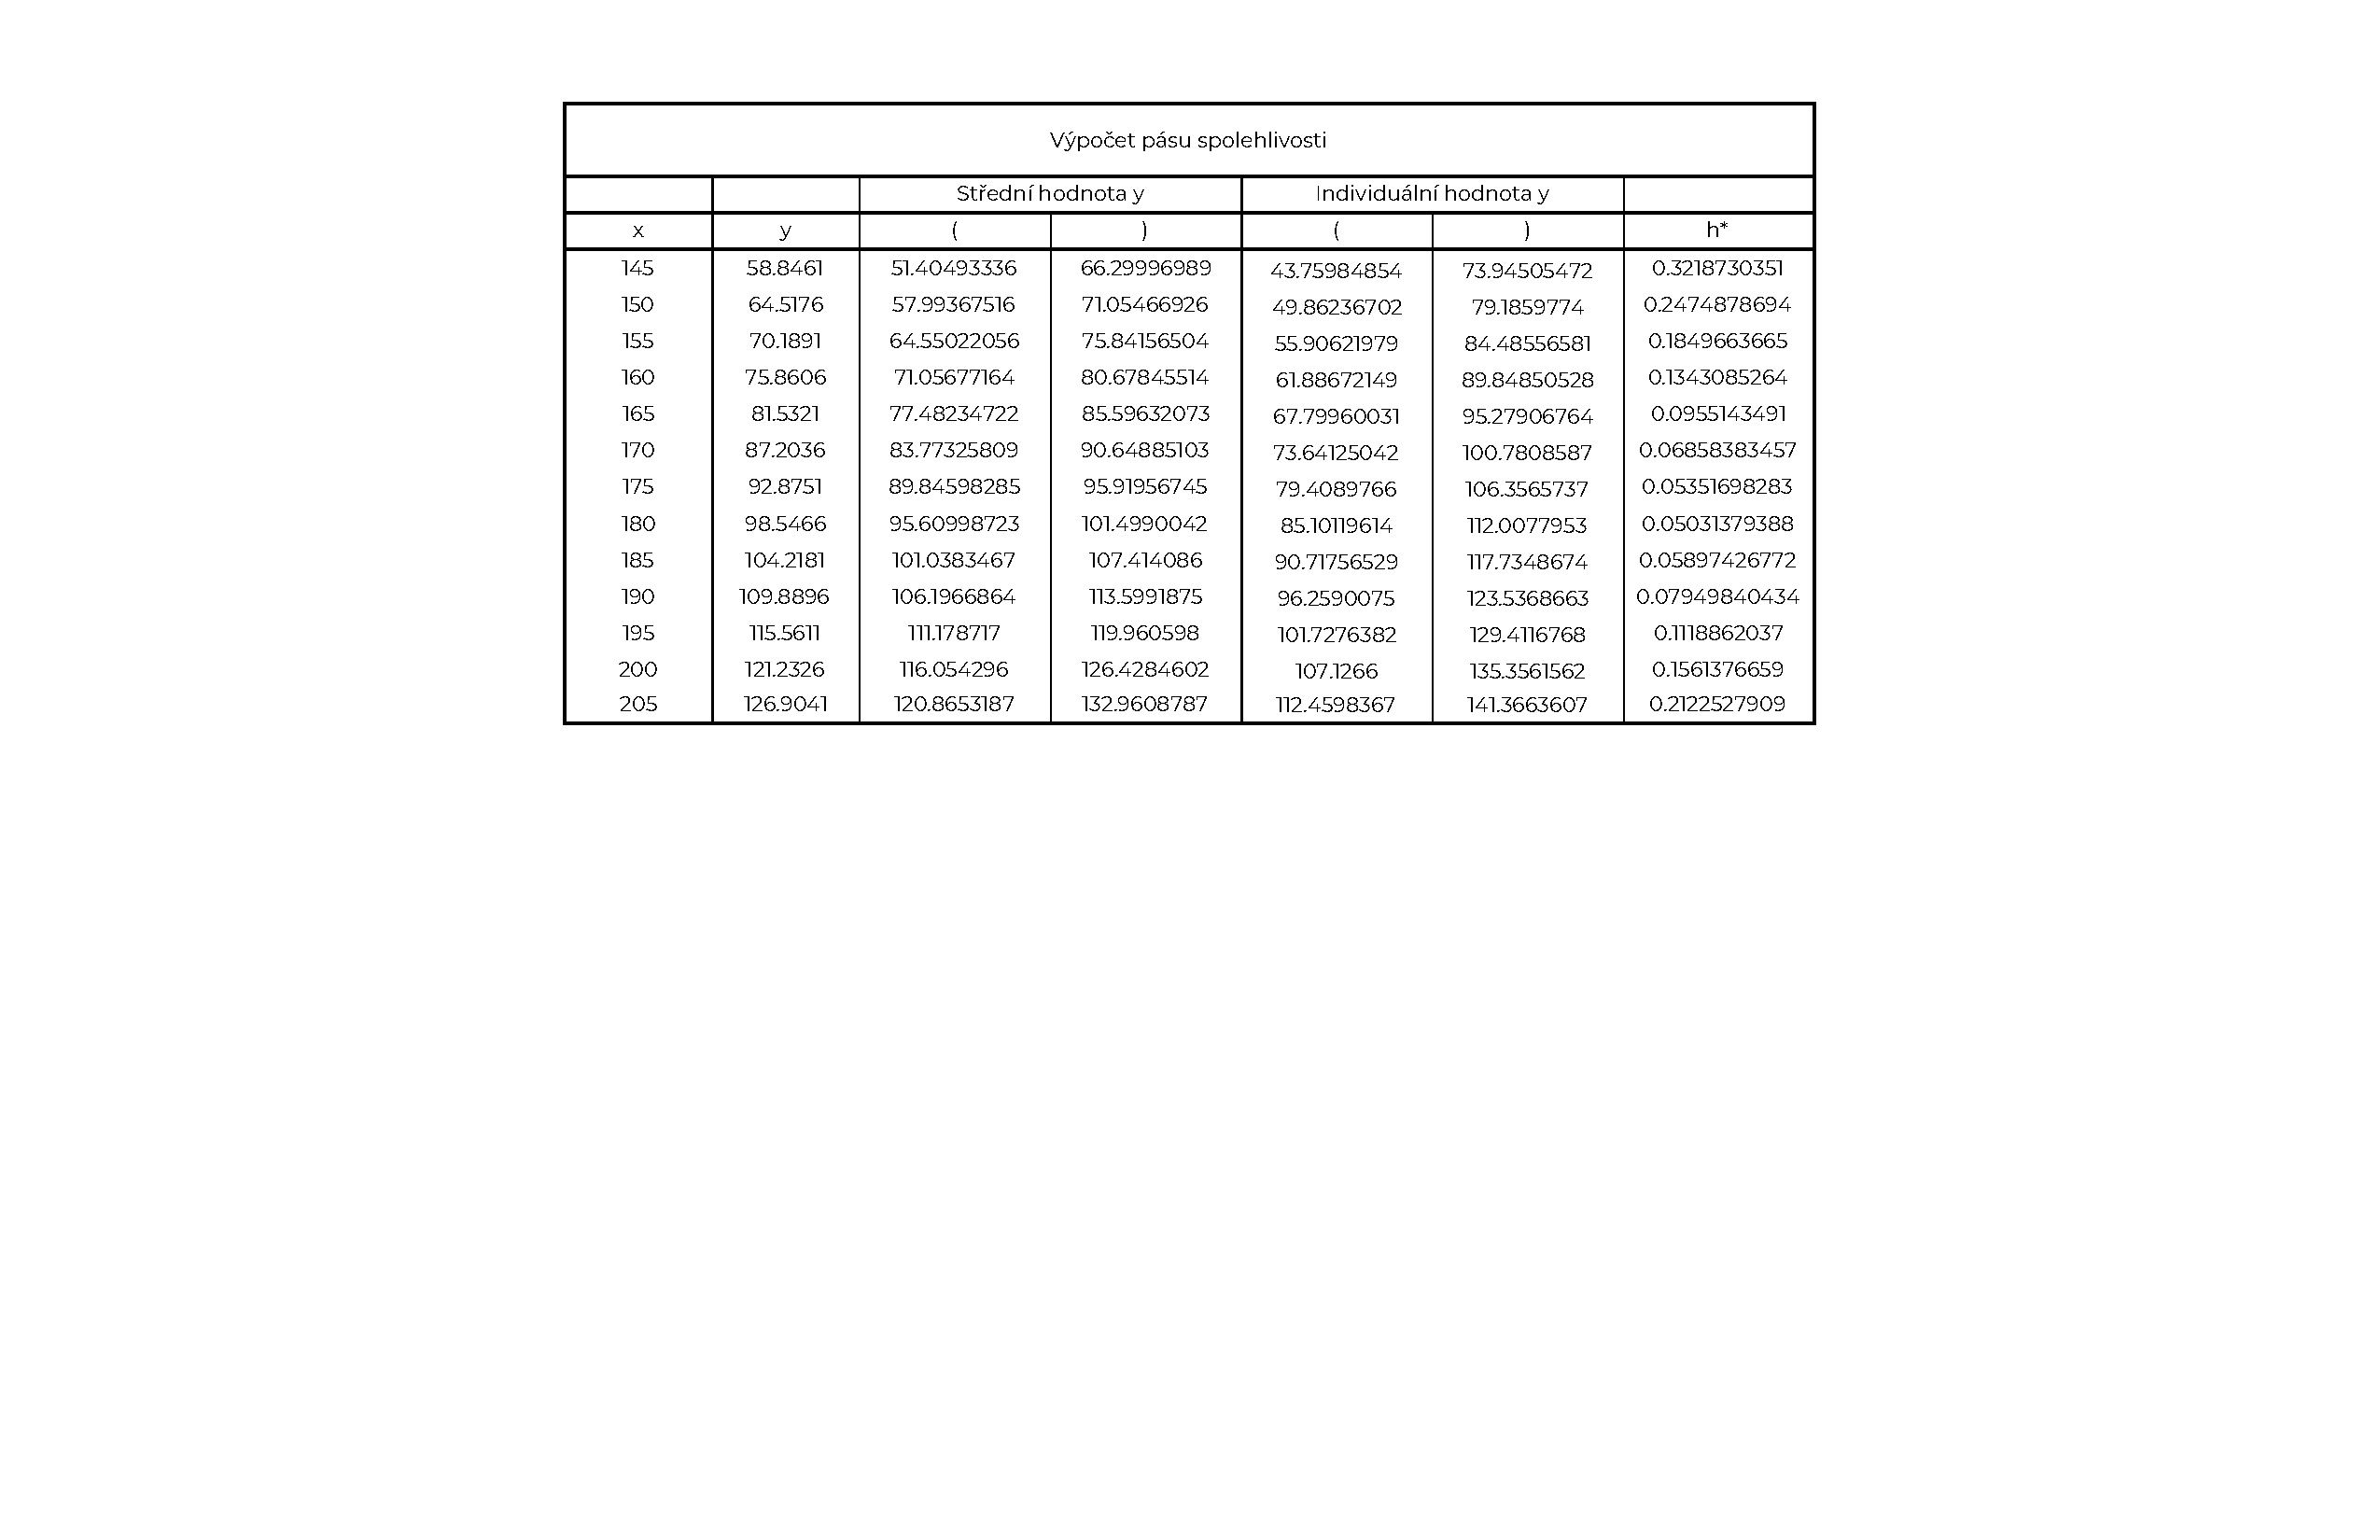
\includegraphics[width=.99\linewidth]{images/2-c-1-crop.pdf}
\end{figure}
\bigskip

\begin{figure}[H]
    \centering
    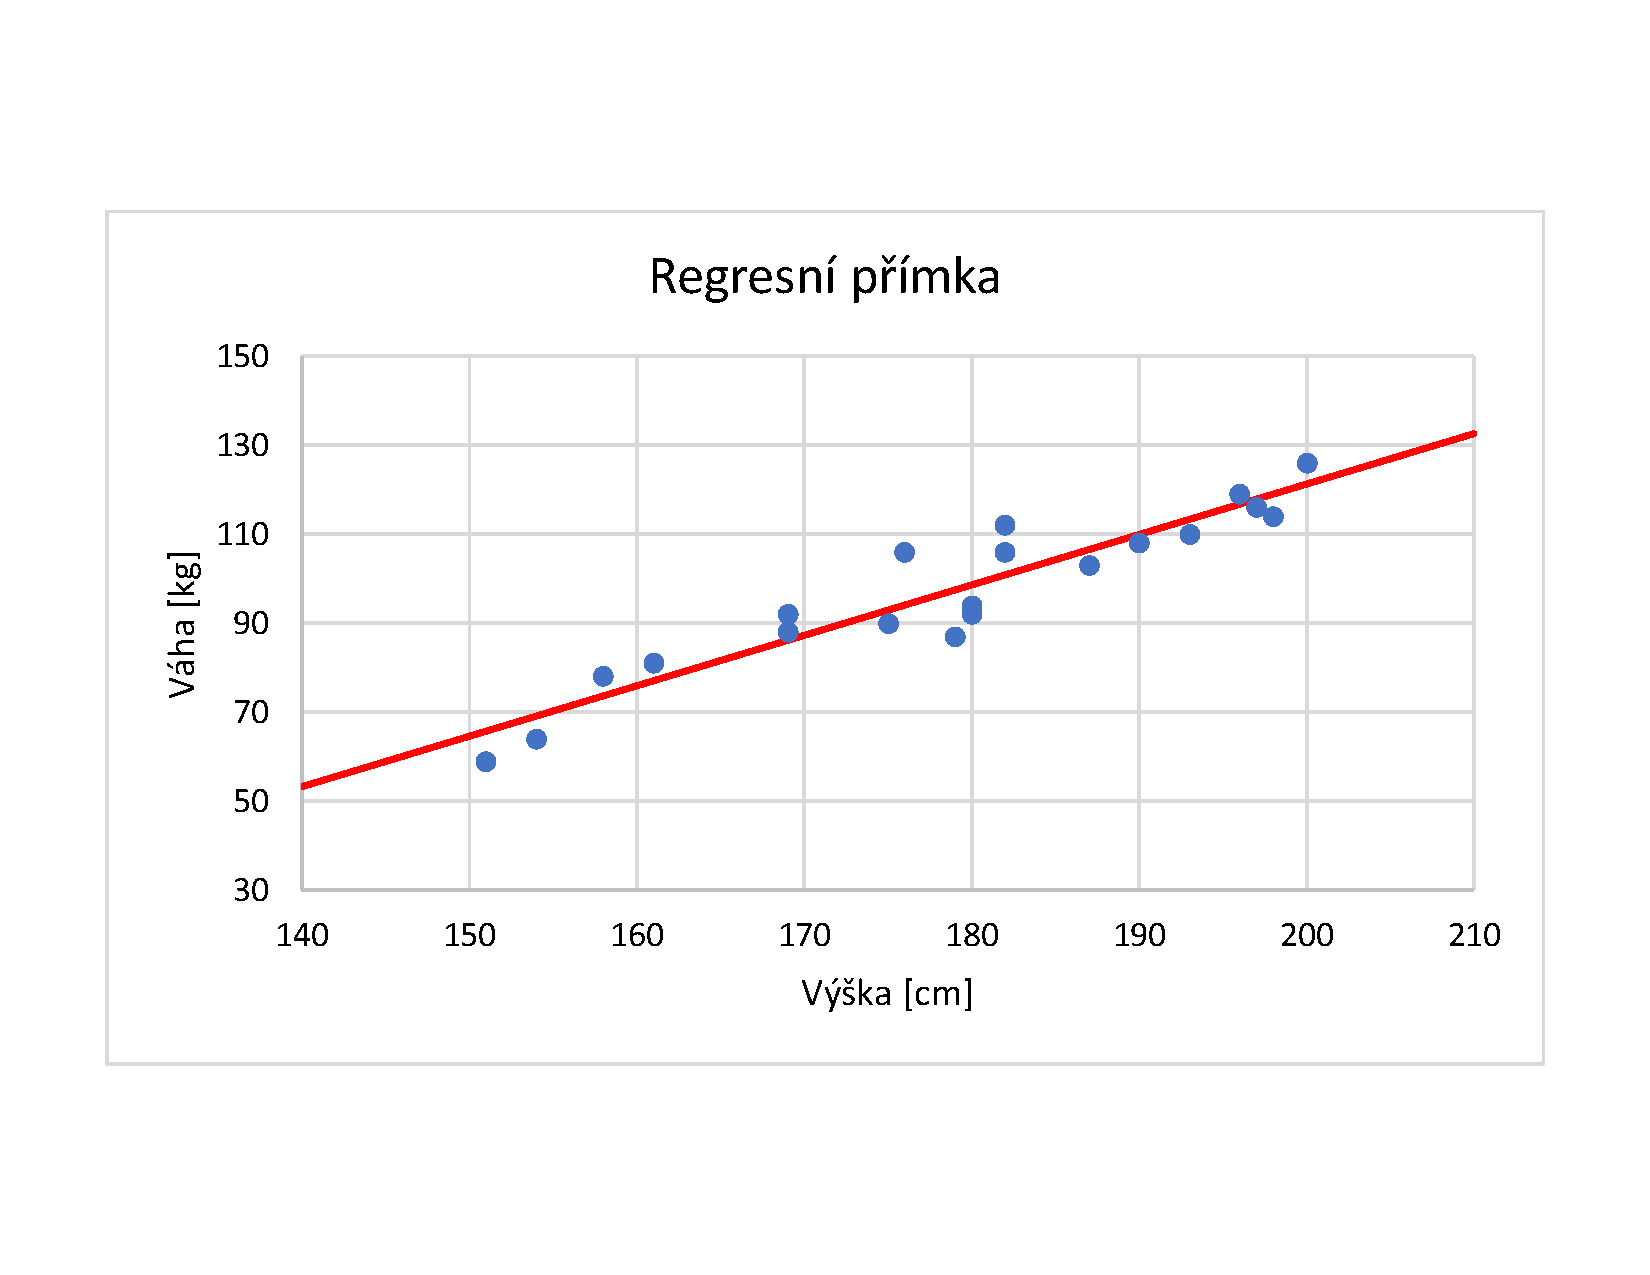
\includegraphics[width=.9\linewidth]{images/2-c-2-crop.pdf}
\end{figure}
\bigskip

\begin{figure}[H]
    \centering
    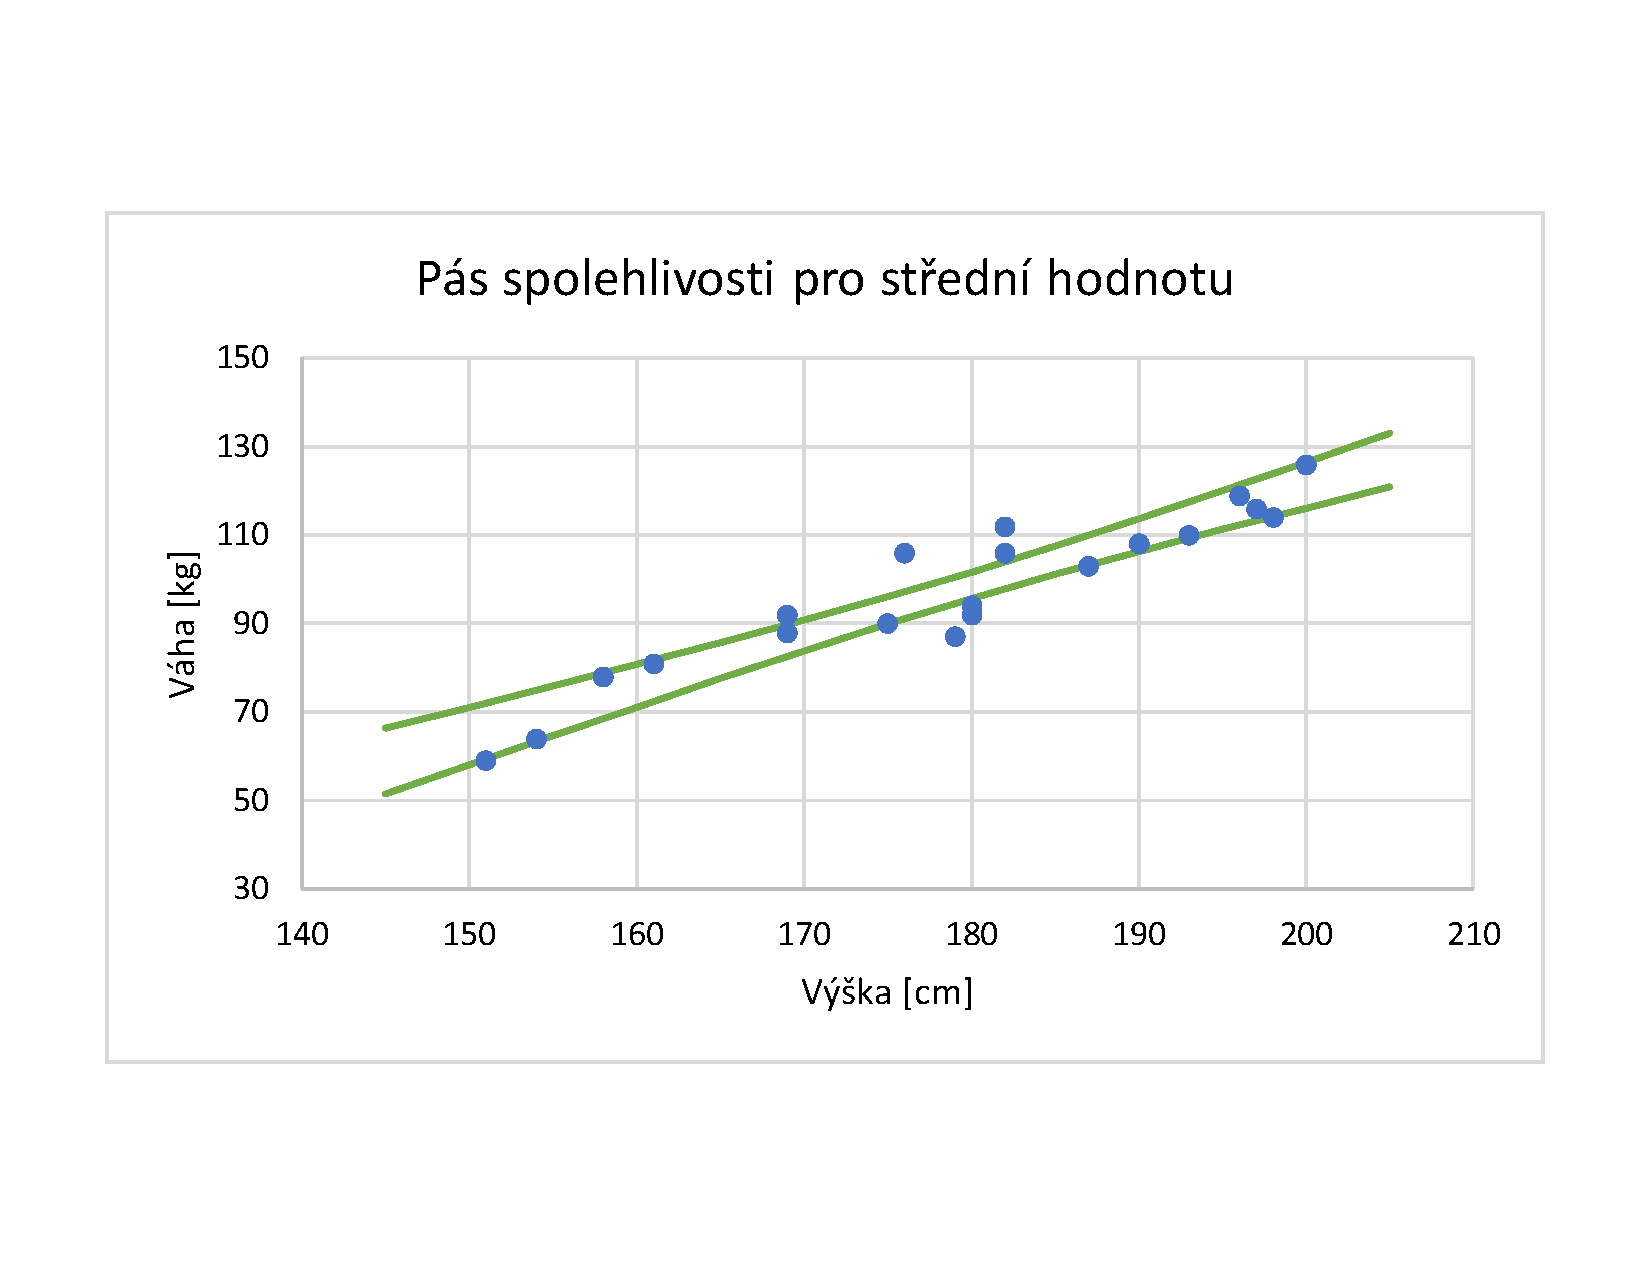
\includegraphics[width=.9\linewidth]{images/2-c-3-crop.pdf}
\end{figure}
\bigskip

\begin{figure}[H]
    \centering
    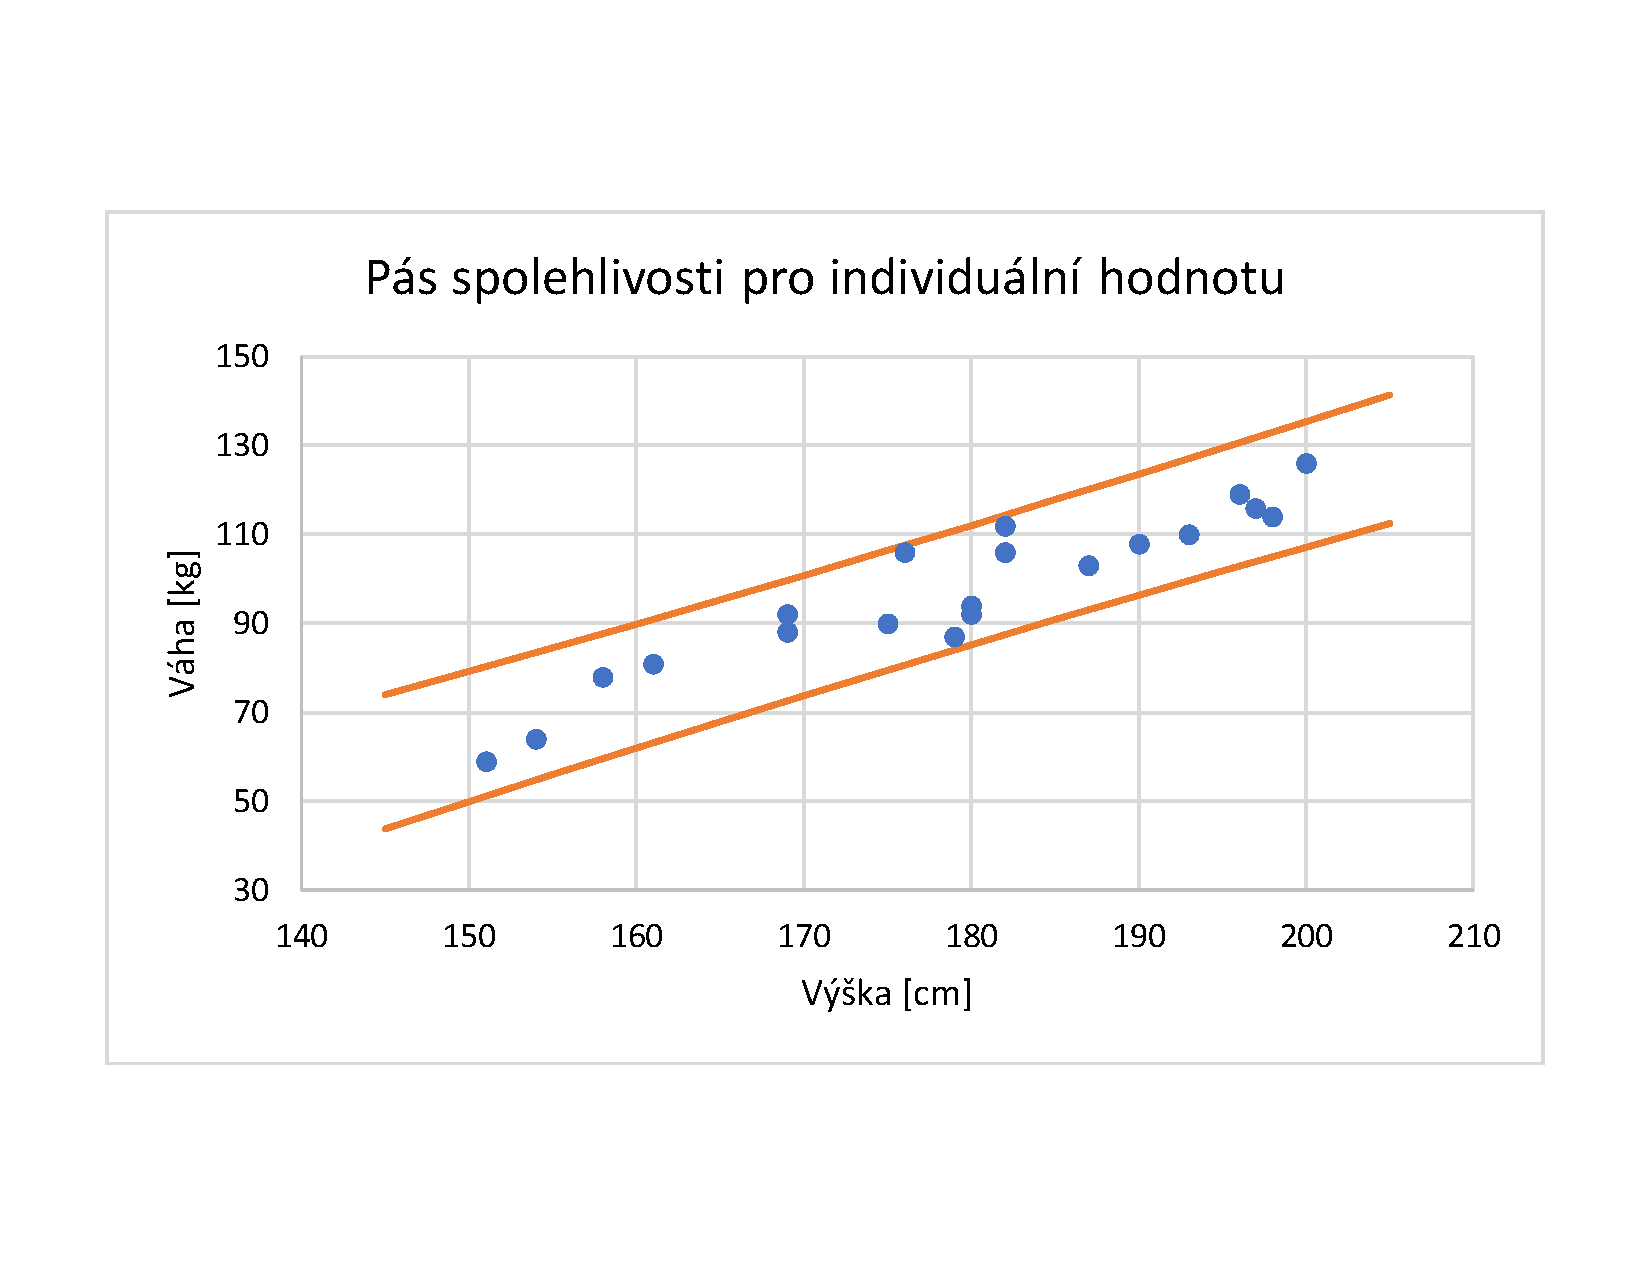
\includegraphics[width=.9\linewidth]{images/2-c-4-crop.pdf}
\end{figure}

%%%%%%%%%%%%%%%%%%%%%%%%%%%%%%%%%%%%%%%%%%%%%%%%%%%%%%%%%%%%%%%%%%%%%

\end{document}
